\documentclass[12pt,a4paper,twoside]{article}

% ------------------------------------------------------------------ pacotes
\usepackage[T1]{fontenc}
\usepackage[utf8]{inputenc}
\usepackage[brazil]{babel}
\usepackage{lmodern}
\usepackage{microtype}
\usepackage[a4paper,margin=2.5cm]{geometry}
\usepackage{amsmath,amssymb,amsthm,bm}
\usepackage{graphicx}
\usepackage{booktabs,array,tabularx,multirow}
\usepackage{caption,subcaption}
\usepackage{xcolor}
\usepackage{tikz}
\usetikzlibrary{arrows.meta,angles,quotes,calc,patterns,babel}
\usepackage[output-decimal-marker={,}, group-separator={.}, range-phrase={ a }, list-final-separator={ e }, list-pair-separator={ e }, list-separator={; }]{siunitx}
\usepackage{enumitem}
\usepackage{csquotes}
\usepackage[style=abnt,backend=biber]{biblatex}
\addbibresource{referencias.bib}
\usepackage{fancyhdr}
\usepackage{setspace}
\usepackage{longtable}
\usepackage{indentfirst}
\setlength{\parindent}{1.5em}
\onehalfspacing
\pagestyle{fancy}
\fancyhf{}
\fancyhead[LE,RO]{Relatório Parcial}
\fancyhead[RE,LO]{PMR3220 - Projeto de Mecanismos}
\fancyfoot[LE,RO]{\thepage}
\fancyfoot[RE,LO]{\textit{\nouppercase{\leftmark}}}
\renewcommand{\sectionmark}[1]{\markboth{#1}{}}
\renewcommand{\headrulewidth}{0.4pt}
\renewcommand{\footrulewidth}{0.4pt}
\usepackage[hidelinks]{hyperref}
\usepackage[brazilian,capitalise,noabbrev]{cleveref}
\usepackage{listings}

\lstset{basicstyle=\ttfamily\footnotesize, breaklines=true, frame=single,
        literate={á}{{\'a}}1 {ã}{{\~a}}1 {é}{{\'e}}1 {ç}{{\c{c}}}1 {õ}{{\~o}}1 {í}{{\'i}}1 {ó}{{\'o}}1}

% Arquivo gerado automaticamente por scripts/gera_valores_tex.py -- nao editar
\newcommand{\Qx}{67{,}4}
\newcommand{\Qy}{\ensuremath{-}97{,}8}
\newcommand{\Nx}{\ensuremath{-}6{,}6}
\newcommand{\Ny}{\ensuremath{-}24{,}6}
\newcommand{\Cx}{\ensuremath{-}7{,}6}
\newcommand{\Cy}{\ensuremath{-}14{,}0}
\newcommand{\Lx}{\ensuremath{-}28{,}4}
\newcommand{\Ly}{\ensuremath{-}24{,}3}
\newcommand{\Px}{39{,}6}
\newcommand{\Py}{\ensuremath{-}419{,}0}
\newcommand{\rCL}{23{,}2}
\newcommand{\rCQ}{112{,}5}
\newcommand{\rQN}{104{,}1}
\newcommand{\rLN}{21{,}8}
\newcommand{\mumin}{42{,}5}
\newcommand{\mumax}{89{,}9}
\newcommand{\grashof}{não satisfaz}
\newcommand{\grashofs}{21{,}8}
\newcommand{\grashofp}{23{,}2}
\newcommand{\grashofq}{104{,}1}
\newcommand{\grashofl}{112{,}5}
\newcommand{\grashofsl}{134{,}3}
\newcommand{\grashofpq}{127{,}3}
\newcommand{\grashofsinal}{>}
\newcommand{\ciOx}{1{,}9}
\newcommand{\ciOy}{\ensuremath{-}24{,}7}
\newcommand{\ciFx}{\ensuremath{-}32{,}3}
\newcommand{\ciFy}{\ensuremath{-}21{,}0}
\newcommand{\phimax}{132{,}0}
\newcommand{\frA}{307}
\newcommand{\phiA}{0{,}0}
\newcommand{\frB}{390}
\newcommand{\phiB}{51{,}7}
\newcommand{\frC}{423}
\newcommand{\phiC}{97{,}2}
\newcommand{\frD}{456}
\newcommand{\phiD}{131{,}9}
\newcommand{\precA}{307}
\newcommand{\precB}{423}
\newcommand{\precC}{456}
\newcommand{\cheque}{390}
\newcommand{\phicheque}{51{,}7}
\newcommand{\errcheque}{0{,}7}
\newcommand{\JPmin}{356}
\newcommand{\JPmax}{367}
\newcommand{\JPvar}{3}
\newcommand{\Jx}{2{,}7}
\newcommand{\Jy}{\ensuremath{-}62{,}2}
\newcommand{\deslO}{60}
\newcommand{\rmaxelo}{112{,}5}
\newcommand{\dalphaA}{\ensuremath{-}97{,}2}
\newcommand{\dalphaB}{\ensuremath{-}131{,}9}
\newcommand{\ddeltaAx}{16{,}7}
\newcommand{\ddeltaAy}{\ensuremath{-}37{,}2}
\newcommand{\ddeltaBx}{2{,}0}
\newcommand{\ddeltaBy}{\ensuremath{-}59{,}9}
\newcommand{\dbetaA}{\ensuremath{-}88{,}0}
\newcommand{\dbetaB}{\ensuremath{-}116{,}0}
\newcommand{\dgamA}{\ensuremath{-}8{,}0}
\newcommand{\dgamB}{\ensuremath{-}40{,}0}
\newcommand{\dWx}{75{,}0}
\newcommand{\dWy}{\ensuremath{-}83{,}8}
\newcommand{\dZx}{\ensuremath{-}67{,}4}
\newcommand{\dZy}{97{,}8}
\newcommand{\dUx}{21{,}8}
\newcommand{\dUy}{\ensuremath{-}0{,}3}
\newcommand{\dSx}{6{,}6}
\newcommand{\dSy}{24{,}6}
\newcommand{\tabelaposes}{234 $\dagger$ & 15{,}4 & 2{,}1 & 1{,}4 & \ensuremath{-}70{,}7 & \ensuremath{-}413{,}1 & 359 \\
307 $\star$ & 0{,}0 & 0{,}0 & 0{,}0 & 39{,}6 & \ensuremath{-}419{,}0 & 359 \\
390 $\circ$ & 51{,}7 & 17{,}3 & \ensuremath{-}12{,}9 & \ensuremath{-}287{,}1 & \ensuremath{-}303{,}5 & 367 \\
423 $\star$ & 97{,}2 & 16{,}7 & \ensuremath{-}37{,}2 & \ensuremath{-}404{,}0 & \ensuremath{-}24{,}3 & 356 \\
456 $\star$ & 131{,}9 & 2{,}0 & \ensuremath{-}59{,}9 & \ensuremath{-}336{,}3 & 190{,}5 & 361 \\
561 $\dagger$ & 155{,}1 & \ensuremath{-}30{,}4 & \ensuremath{-}60{,}4 & \ensuremath{-}242{,}5 & 303{,}1 & 345 \\}
\newcommand{\tabelacombos}{307, 423, 456 & 390 & 0{,}71 & 42{,}5 \\
307, 390, 456 & 423 & 0{,}93 & 38{,}6 \\
307, 390, 423 & 456 & 0{,}99 & 32{,}2 \\}
\newcommand{\mUmA}{9{,}88}
\newcommand{\aUmA}{0{,}207}
\newcommand{\IUmA}{0{,}202}
\newcommand{\mDoisA}{5{,}44}
\newcommand{\bxDoisA}{0{,}258}
\newcommand{\byDoisA}{0{,}031}
\newcommand{\IDoisA}{0{,}172}
\newcommand{\mUmB}{7{,}88}
\newcommand{\aUmB}{0{,}215}
\newcommand{\IUmB}{0{,}165}
\newcommand{\mDoisB}{4{,}22}
\newcommand{\bxDoisB}{0{,}259}
\newcommand{\byDoisB}{0{,}031}
\newcommand{\IDoisB}{0{,}133}
\newcommand{\mUmS}{8{,}00}
\newcommand{\mDoisS}{4{,}88}
\newcommand{\massaOrtese}{2{,}43}
\newcommand{\tabelaortese}{coxa & hastes laterais Al 6061-T6 (2x) & 0{,}216 & (0{,}200; 0{,}000) \\
perna & hastes laterais Al 6061-T6 (2x) & 0{,}243 & (0{,}225; 0{,}000) \\
coxa & braçadeira proximal PP & 0{,}131 & (0{,}100; 0{,}000) \\
coxa & braçadeira distal PP & 0{,}131 & (0{,}300; 0{,}000) \\
perna & braçadeira PP & 0{,}131 & (0{,}150; 0{,}000) \\
perna & palmilha PP + estribo & 0{,}181 & (0{,}450; 0{,}125) \\
coxa & articulação do joelho (aço AISI 304) & 0{,}200 & (0{,}400; 0{,}000) \\
coxa & atuador do joelho (motor + redutor) & 1{,}200 & (0{,}400; 0{,}000) \\}
\newcommand{\tabelatorques}{final I & 80 & 6{,}2 & 13{,}5 \\
final I & 60 & 4{,}7 & 10{,}5 \\
final II & 80 & 40{,}0 & 2{,}8 \\
final II & 60 & 32{,}1 & 2{,}2 \\}
\newcommand{\tabelacinematica}{final I & 9{,}5 & 103{,}0 & 112{,}5 & 14{,}6 & 158{,}6 & 173{,}2 \\
final II & 93{,}8 & 9{,}2 & 103{,}0 & 144{,}4 & 14{,}2 & 158{,}6 \\}
\newcommand{\tqImax}{6{,}2}
\newcommand{\tjImax}{13{,}5}
\newcommand{\tqIImax}{40{,}0}
\newcommand{\tjIImax}{2{,}8}
\newcommand{\wmaxII}{93{,}8}
\newcommand{\wmaxI}{112{,}5}
\newcommand{\repQ}{1{,}645}
\newcommand{\repJ}{1{,}645}
\newcommand{\repmgb}{1{,}645}


\newcommand{\ve}[1]{\bm{#1}}
% --- notacao do metodo matricial (PMR3220) ---
\DeclareMathOperator{\sen}{sen}
\newcommand{\rv}[2]{{}^{#1}\mathbf{r}_{#2}}          % vetor posicao do ponto #2 na base #1
\newcommand{\rvd}[2]{{}^{#1}\dot{\mathbf{r}}_{#2}}
\newcommand{\rvdd}[2]{{}^{#1}\ddot{\mathbf{r}}_{#2}}
\newcommand{\vv}[2]{{}^{#1}\mathbf{v}_{#2}}
\newcommand{\Tm}[2]{{}^{#1}T_{#2}}                   % transformacao homogenea da base #2 para a base #1
\newcommand{\Tmd}[2]{{}^{#1}\dot T_{#2}}
\newcommand{\Tmdd}[2]{{}^{#1}\ddot T_{#2}}
\newcommand{\Rm}[2]{[{}^{#1}R_{#2}]}                 % matriz de rotacao
\newcommand{\Rot}[2]{\mathrm{Rot}(#1,\,#2)}
\newcommand{\hmg}[1]{\begin{bmatrix} #1 \\ 1 \end{bmatrix}}
\newcommand{\hoz}[1]{\begin{bmatrix} #1 \\ 0 \end{bmatrix}}
\newcommand{\Jm}[1]{[J_{#1}]}
\newcommand{\e}{\mathrm{e}}
\newcommand{\dd}{\,\mathrm{d}}
\newtheorem{hipotese}{Hipótese}
\captionsetup{font=small,labelsep=colon}
\numberwithin{equation}{section}

% ------------------------------------------------------------------ capa
\begin{document}
\begin{titlepage}
  \centering
  {\Large\bfseries ESCOLA POLITÉCNICA DA UNIVERSIDADE DE SÃO PAULO\par}
  \vspace{1.2cm}
  {\large\bfseries PMR3220 - Projeto de Mecanismos\par}
  \vspace{0.8cm}
  Prof. Dr. Ricardo Cury Ibrahim\par
  Prof. Dr. Tarcisio Antonio Hess Coelho\par
  \vspace{0.9cm}
  {\bfseries Grupo C\par}
  \vspace{0.5cm}
  \begin{spacing}{1.6}
  André Neme Benedetti - NUSP\par
  André Tsukassa Nishimoto - NUSP\par
  Felipe Wassmer Magina - NUSP\par
  Júlio Cesar de Andrade Oliveira - NUSP\par
  Lucas Sung Il Hong - NUSP\par
  Matheus Moreira de Sousa - NUSP\par
  Matheus Paixão de Sousa - NUSP\par
  Pedro Henrique Brasileiro de Jesus - NUSP\par
  \end{spacing}
  \vspace{0.7cm}
  {\LARGE Relatório Parcial\par}
  \vspace{0.3cm}
  {\bfseries Prótese e órtese de membro inferior\par}
  \vspace{0.8cm}
  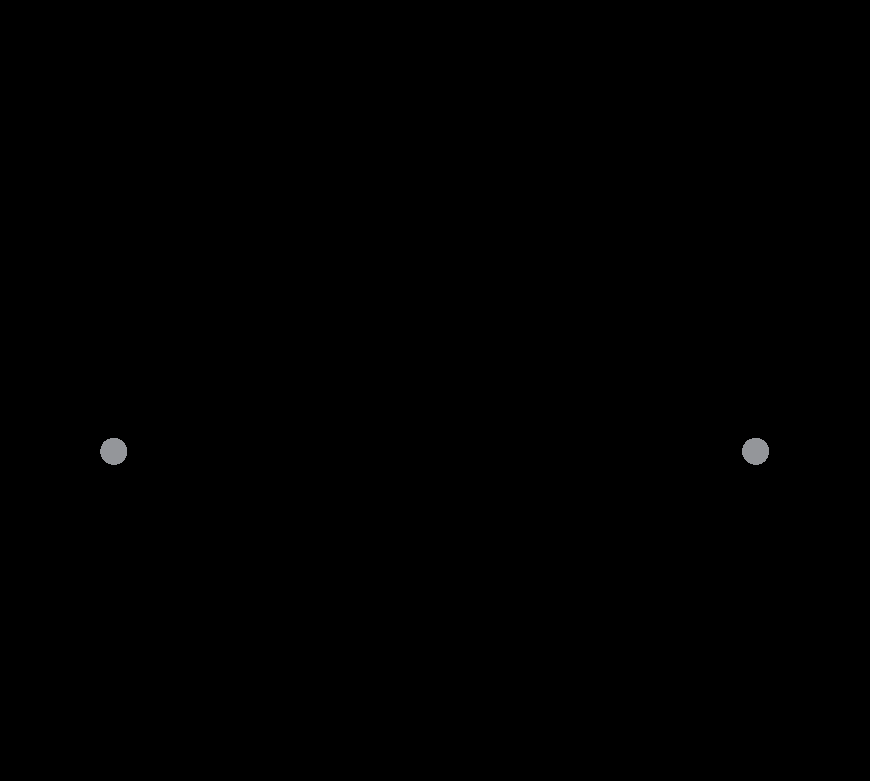
\includegraphics[width=4.2cm]{figuras/rasc_p1_0.png}\par
  \vfill
  {\large\bfseries São Paulo, 7 de outubro de 2026\par}
\end{titlepage}

\pagenumbering{roman}
\listoffigures
\clearpage
\listoftables
\clearpage
\tableofcontents
\clearpage
\pagenumbering{arabic}
\setcounter{page}{5}

\section{Introdução}

O movimento do membro inferior humano resulta da interação entre diferentes segmentos
e articulações, sendo o joelho particularmente importante para a mobilidade entre a
coxa e a perna. Entretanto, seu movimento relativo não pode ser rigorosamente
representado por uma simples junta de revolução: no plano sagital, os côndilos
femorais rolam e deslizam sobre o platô tibial, de modo que o centro instantâneo de
rotação (CIR) descreve uma trajetória -- a \emph{centroide} -- em vez de permanecer fixo
\cite{menschik1974,oconnor1989,dathe2016}. Desde \textcite{menschik1974}, essa cinemática
é modelada por um quadrilátero articulado cruzado, formado pelas fibras isométricas
dos ligamentos cruzados anterior (LCA) e posterior (LCP) e pelos segmentos ósseos que
unem suas inserções \cite{oconnor1989,zavatsky1992}.

Nesse contexto, o projeto de próteses e órteses constitui uma aplicação relevante da
teoria de mecanismos, permitindo reproduzir ou auxiliar movimentos do membro inferior
em situações de amputação ou de comprometimento da capacidade motora -- por exemplo,
após um acidente grave, um acidente vascular cerebral (AVC) ou uma lesão por esforço
intenso. Este trabalho aborda a aplicação de mecanismos articulados a esses problemas
em duas partes, propostas no enunciado da disciplina (\cref{fig:enunciado}):

\begin{enumerate}[label=\textbf{Parte \Roman*.},leftmargin=*]
  \item \textbf{Prótese de joelho e perna}: síntese dimensional de um quadrilátero
  articulado plano cujo acoplador (conjunto perna--pé artificial) reproduza o movimento
  relativo entre a perna e a coxa, medido experimentalmente em um integrante do grupo,
  e construção de uma maquete para avaliar qualitativamente o funcionamento.
  \item \textbf{Órtese de membro inferior}: análise cinemática, por interpolação
  polinomial de 5º grau, e análise dinâmica de uma órtese para um indivíduo de
  \SIrange{60}{80}{kg} com a musculatura inativa, determinando os torques dos atuadores
  do joelho e do quadril.
\end{enumerate}

\begin{figure}[htbp]
  \centering
  \begin{subfigure}[b]{0.40\textwidth}
    \centering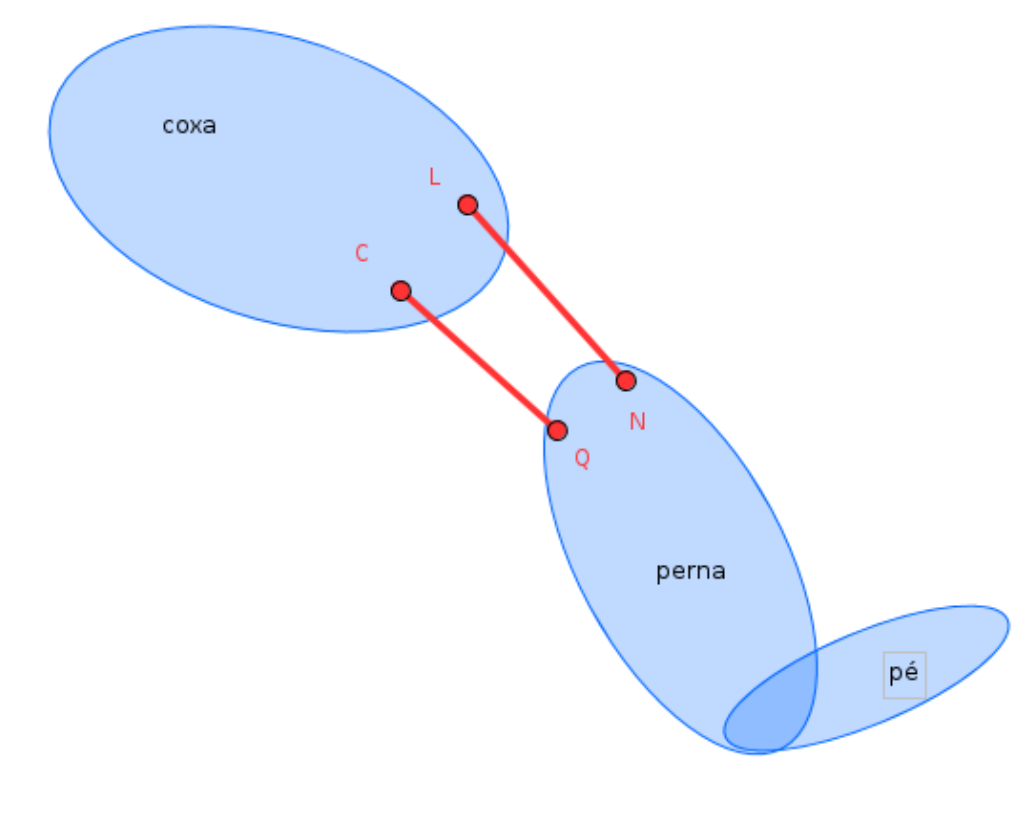
\includegraphics[width=\textwidth]{figuras/enunciado_fig1.png}
    \caption{Diagrama cinemático: pivôs $C$, $L$ na coxa e $Q$, $N$ na perna.}
  \end{subfigure}\hfill
  \begin{subfigure}[b]{0.56\textwidth}
    \centering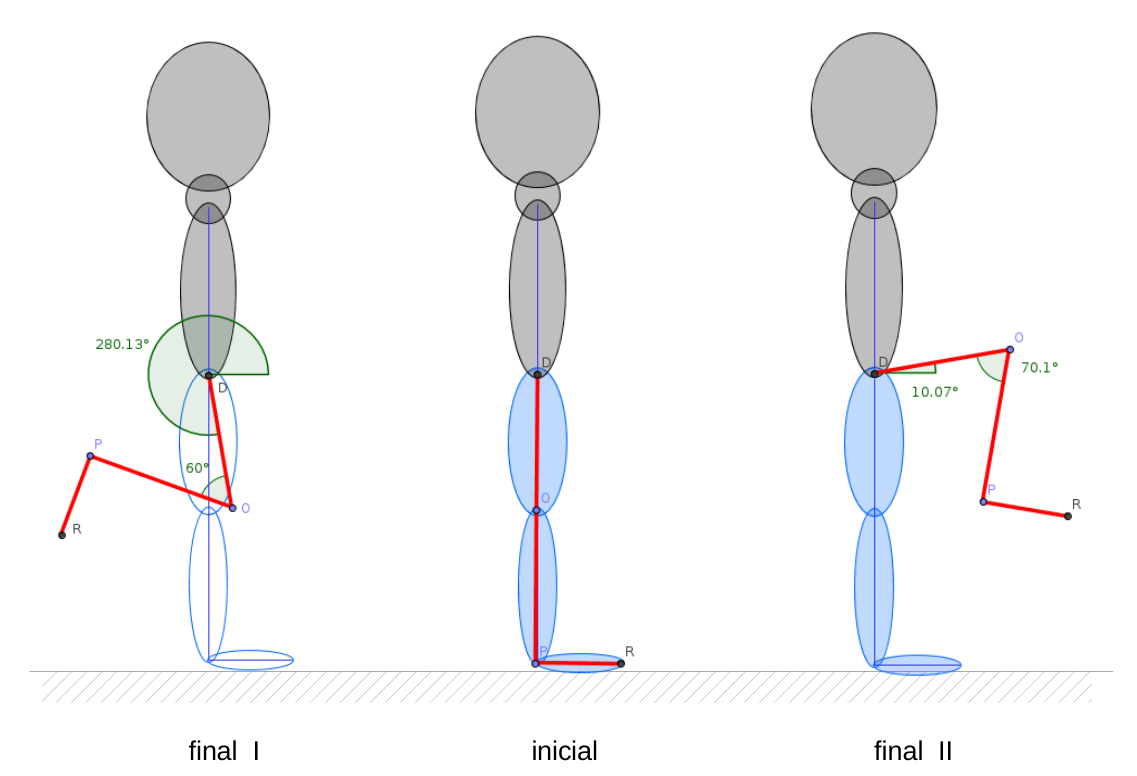
\includegraphics[width=\textwidth]{figuras/enunciado_fig2.png}
    \caption{Configurações final I, inicial e final II da órtese.}
  \end{subfigure}
  \caption{Figuras do enunciado (reproduzidas).}
  \label{fig:enunciado}
\end{figure}

\section{Objetivos}

\begin{itemize}
  \item Desenvolver a síntese dimensional de um mecanismo quadrilátero articulado,
  capaz de reproduzir de forma aproximada o movimento relativo entre a coxa e o
  conjunto perna--pé de uma prótese de membro inferior.
  \item Determinar as dimensões e as posições das articulações do mecanismo, utilizando
  como referência as posições do membro inferior obtidas experimentalmente.
  \item Construir uma maquete que permita avaliar qualitativamente o funcionamento do
  mecanismo sintetizado.
  \item Realizar a análise cinemática de uma órtese para membro inferior, determinando
  as orientações, velocidades e acelerações angulares dos segmentos ao longo de um
  ciclo de movimento.
  \item Realizar a análise dinâmica do sistema, determinando os torques necessários nos
  atuadores do joelho e da articulação entre a coxa e o tronco para a execução do
  movimento considerado, com massas e momentos de inércia obtidos de dados
  antropométricos e dos materiais selecionados para a órtese.
\end{itemize}

Em todas as deduções, os passos intermediários são mostrados, de modo que os
resultados possam ser reproduzidos à mão. Os cálculos foram implementados em Python
(NumPy, SciPy, SymPy e Matplotlib), e os valores numéricos citados no texto são lidos
automaticamente dos resultados, o que garante consistência entre cálculo e relatório
(\cref{sec:anexos}).

\section{Fundamentação teórica}\label{cap:teoria1}

\subsection{Notação}\label{sec:notacao}

A modelagem cinemática segue o \emph{método matricial} adotado na disciplina, baseado em
transformações homogêneas. A cada elo $i$ associa-se uma base (sistema de referência)
$O_iX_iY_iZ_i$, de versores $\mathbf i_i$, $\mathbf j_i$, $\mathbf k_i$; a base $0$ é fixa. As
convenções são:
\begin{itemize}
  \item $\rv{A}{P}$: vetor posição do ponto $P$ escrito na base $A$ (o sobrescrito à esquerda
  indica a base);
  \item $\Rm{A}{B} = [\,{}^{A}\mathbf i_B,\ {}^{A}\mathbf j_B,\ {}^{A}\mathbf k_B\,]$: matriz de rotação
  cujas colunas são os versores da base $B$ escritos na base $A$, com
  $\Rm{B}{A} = \Rm{A}{B}^{-1} = \Rm{A}{B}^{\mathsf T}$;
  \item rotação simples de ângulo $\gamma$ em torno do eixo $z_B$ (movimento plano):
  \begin{equation}
    \Rm{A}{B} = \Rot{\gamma}{z_B} =
    \begin{bmatrix} \cos\gamma & -\sen\gamma & 0\\ \sen\gamma & \cos\gamma & 0\\ 0 & 0 & 1 \end{bmatrix},
    \qquad
    \begin{aligned}
      \mathbf i_B &= \cos\gamma\,\mathbf i_A + \sen\gamma\,\mathbf j_A,\\
      \mathbf j_B &= -\sen\gamma\,\mathbf i_A + \cos\gamma\,\mathbf j_A,\\
      \mathbf k_B &= \mathbf k_A;
    \end{aligned}
  \end{equation}
  no plano, usa-se apenas o bloco $2\times2$ superior;
  \item mudança de base de um ponto: $\rv{A}{P} = \Rm{A}{B}\,\rv{B}{P} + \rv{A}{O_B}$, ou, na forma
  homogênea,
  \begin{equation}
    \hmg{\rv{A}{P}} = \Tm{A}{B}\hmg{\rv{B}{P}},
    \qquad
    \Tm{A}{B} = \left[\begin{array}{c|c} \Rm{A}{B} & \rv{A}{O_B} \\ \hline \mathbf 0 & 1 \end{array}\right],
    \label{eq:homogenea}
  \end{equation}
  e, para uma cadeia de elos, $\Tm{0}{n} = \Tm{0}{1}\,\Tm{1}{2}\cdots\Tm{n-1}{n}$;
  \item abreviações: $c_i = \cos\theta_i$, $s_i = \sen\theta_i$, $c_{ij} = \cos(\theta_i+\theta_j)$,
  $s_{ij} = \sen(\theta_i+\theta_j)$; o ângulo $\theta_i$ da junta $i$ é medido do eixo $X_{i-1}$ ao
  eixo $X_i$ (ângulo \emph{relativo}), positivo no sentido anti-horário;
  \item produto vetorial na forma matricial: $\mathbf a \times \mathbf b = \tilde{\mathbf a}\,\mathbf b$, com
  $\tilde{\mathbf a} = \begin{bmatrix} 0 & -a_z & a_y\\ a_z & 0 & -a_x\\ -a_y & a_x & 0\end{bmatrix}$.
\end{itemize}

\section{Objetivos e organização do relatório}

O objetivo geral é aplicar as ferramentas de análise e síntese de mecanismos da
disciplina a um problema de engenharia de reabilitação: substituir (prótese) ou
auxiliar (órtese) o movimento do membro inferior. Os objetivos específicos são:
\begin{enumerate}[label=(\alph*)]
  \item descrever o movimento relativo perna--coxa e dimensionar um quadrilátero
  articulado que o reproduza (Parte~I);
  \item gerar, por interpolação polinomial, trajetórias suaves para um ciclo de
  movimento do membro com órtese e obter as orientações, velocidades e acelerações
  angulares dos elos (Parte~II);
  \item calcular os torques que os atuadores do quadril e do joelho precisam fornecer,
  com massas e inércias obtidas de dados antropométricos e dos materiais da órtese,
  e verificar a estrutura da órtese (Parte~II).
\end{enumerate}
A Parte~I ocupa os \cref{cap:teoria1,cap:metodos1,cap:resultados1,cap:maquete}: a
fundamentação e a formulação matemática da síntese, o protocolo de medição, os
resultados e a maquete. A Parte~II ocupa os \cref{cap:cinematica,cap:parametros,cap:dinamica,cap:resultados2,cap:dimensionamento}:
a cinemática, os parâmetros de massa, a dinâmica, os resultados e o dimensionamento.
Em todas as deduções, cada passo intermediário é mostrado, de modo que o leitor possa
reproduzir os resultados à mão.

\subsection{Quadrilátero articulado e o joelho policêntrico}

Um quadrilátero articulado plano possui quatro elos ligados por quatro juntas de
revolução e, pelo critério de Grübler, um grau de liberdade:
\begin{equation}
  M = 3(n-1) - 2j_1 - j_2 = 3(4-1) - 2\cdot 4 - 0 = 1 .
\end{equation}
No joelho protético (\cref{fig:enunciado}a) o elo fixo é a coxa (pivôs $C$ e $L$),
as manivelas/balancins são $CQ$ e $LN$, e o \emph{acoplador} é a perna (pivôs $Q$ e $N$),
ao qual se fixa rigidamente o pé. Como o acoplador executa um movimento plano geral,
seu CIR relativo à coxa -- o polo $I_{13}$ -- é, pelo teorema de Aronhold--Kennedy, a
intersecção das retas $CQ$ e $LN$ e se desloca à medida que o joelho flexiona, tal como
no joelho natural \cite{norton2010,radcliffe1994}. Joelhos protéticos de quatro barras
exploram essa propriedade: com o CIR alto e posterior na extensão, obtém-se
estabilidade voluntária na fase de apoio; com o CIR migrando na flexão, obtém-se
encurtamento aparente da perna na fase de balanço \cite{radcliffe1994}.

A condição de Grashof classifica o tipo de movimento possível. Sendo $s$ e $l$ os
comprimentos do menor e do maior elo e $p$, $q$ os demais,
\begin{equation}
  s + l \le p + q \quad\Longrightarrow\quad \text{pelo menos um elo dá voltas completas.}
  \label{eq:grashof}
\end{equation}
Na prótese, a flexão útil está limitada a cerca de \SI{120}{\degree}; logo, um mecanismo
não Grashof (triplo balancim) é aceitável, desde que nenhuma configuração de ponto
morto ocorra dentro dessa faixa. A qualidade da transmissão de forças é avaliada pelo
ângulo de transmissão $\mu$ -- ângulo agudo entre o acoplador e o balancim de saída --,
recomendando-se $\mu \ge \SI{30}{\degree}$ \cite{norton2010}.

\subsection{Bases e análise de posição do quadrilátero (cadeia fechada)}\label{sec:cadeia_fechada}

A \cref{fig:quadrilatero} mostra as bases adotadas, seguindo a convenção da
\cref{sec:notacao}. A base $0$ (fixa) está presa à coxa, com origem no centro do joelho em
extensão, $X_0$ para a frente (anterior) e $Y_0$ para cima (proximal). As bases $1$, $2$ e $3$
estão presas, respectivamente, ao elo $CQ$ (origem em $C$, $X_1$ ao longo de $CQ$), ao
acoplador (origem em $Q$, $X_2$ ao longo de $QN$) e ao elo $LN$ (origem em $L$, $X_3$ ao longo
de $LN$). A base $4$ também está presa à perna, com origem no ponto de referência do
joelho e $Y_4$ ao longo do eixo da perna (é a base em que se fazem as medições). Os
comprimentos são $\ell_0 = \overline{CL}$, $\ell_1 = \overline{CQ}$, $\ell_2 = \overline{QN}$ e
$\ell_3 = \overline{LN}$.

\begin{figure}[htbp]
  \centering
  \begin{tikzpicture}[scale=1.35, >=Stealth]
    \coordinate (C) at (0,0);
    \coordinate (L) at (3,0.6);
    \coordinate (Q) at ({1.6*cos(115)},{1.6*sin(115)});
    \coordinate (N) at ($(L)+({2.4*cos(128)},{2.4*sin(128)})$);
    \draw[thick] (C) -- node[left, pos=0.6] {$\ell_1$} (Q) -- node[above left, pos=0.6] {$\ell_2$} (N) -- node[right] {$\ell_3$} (L);
    \draw[thick,dashed,gray] (C) -- node[below] {$\ell_0$} (L);
    \foreach \p in {C,Q,N,L} \draw[fill=white] (\p) circle (0.06);
    \node[below left] at (C) {$C$}; \node[below right] at (L) {$L$};
    \node[left] at (Q) {$Q$}; \node[above right] at (N) {$N$};
    % base 0
    \draw[->,thick] (-1.2,-0.8) -- (-0.4,-0.8) node[below] {$X_0$};
    \draw[->,thick] (-1.2,-0.8) -- (-1.2,0) node[left] {$Y_0$};
    % base 1
    \draw[->,teal] (C) -- ($(C)!0.45!(Q)$) node[right=2pt] {$X_1$};
    \draw[dashed,blue] (C) -- (1,0) coordinate (Ce);
    \pic[draw,->,blue,"$\theta_1$",angle radius=0.5cm,angle eccentricity=1.45] {angle=Ce--C--Q};
    % base 2
    \coordinate (Qe) at ($(Q)!-0.5!(C)$);
    \draw[dashed,blue] (Q) -- (Qe);
    \draw[->,teal] (Q) -- ($(Q)!0.3!(N)$) node[below] {$X_2$};
    \pic[draw,->,blue,"$\theta_2$",angle radius=0.45cm,angle eccentricity=1.5] {angle=N--Q--Qe};
    % base 3
    \draw[dashed,blue] (L) -- ($(L)+(0.8,0.16)$) coordinate (Le);
    \draw[->,teal] (L) -- ($(L)!0.25!(N)$) node[left] {$X_3$};
    \pic[draw,->,blue,"$\theta_3$",angle radius=0.45cm,angle eccentricity=1.5] {angle=Le--L--N};
    \node[gray] at (0.4,2.8) {perna (acoplador)};
    \node[gray] at (1.5,-0.6) {coxa (elo fixo 0)};
  \end{tikzpicture}
  \caption{Quadrilátero articulado do joelho: bases, ângulos e comprimentos (a base $1$ e a
  base $3$ têm os ângulos medidos a partir de $X_0$; $\theta_2$ é medido a partir de $X_1$).}
  \label{fig:quadrilatero}
\end{figure}

As transformações homogêneas \eqref{eq:homogenea} de cada elo são
\begin{equation}
  \Tm{0}{1} = \left[\begin{array}{cc|c} c_1 & -s_1 & {}^0x_C\\ s_1 & c_1 & {}^0y_C\\ \hline 0 & 0 & 1\end{array}\right],\quad
  \Tm{1}{2} = \left[\begin{array}{cc|c} c_2 & -s_2 & \ell_1\\ s_2 & c_2 & 0\\ \hline 0 & 0 & 1\end{array}\right],\quad
  \Tm{0}{3} = \left[\begin{array}{cc|c} c_3 & -s_3 & {}^0x_L\\ s_3 & c_3 & {}^0y_L\\ \hline 0 & 0 & 1\end{array}\right],
\end{equation}
com $\rv{2}{N} = [\ell_2\ \ 0]^{\mathsf T}$ e $\rv{3}{N} = [\ell_3\ \ 0]^{\mathsf T}$. O ponto $N$ pertence
simultaneamente ao ramo $0\text{--}1\text{--}2$ e ao ramo $0\text{--}3$ da cadeia. Pelo ramo
$0\text{--}1\text{--}2$, multiplica-se primeiro o ponto pela matriz mais à direita:
\begin{equation*}
  \Tm{1}{2}\hmg{\rv{2}{N}} = \begin{bmatrix} \ell_2 c_2 + \ell_1 \\ \ell_2 s_2 \\ 1\end{bmatrix},
  \qquad
  \Tm{0}{1}\begin{bmatrix} \ell_2 c_2 + \ell_1 \\ \ell_2 s_2 \\ 1\end{bmatrix}
  = \begin{bmatrix} {}^0x_C + \ell_1 c_1 + \ell_2(c_1c_2 - s_1s_2) \\ {}^0y_C + \ell_1 s_1 + \ell_2(s_1c_2 + c_1s_2) \\ 1\end{bmatrix},
\end{equation*}
e as identidades $c_1c_2 - s_1s_2 = c_{12}$ e $s_1c_2 + c_1s_2 = s_{12}$ simplificam o resultado.
Igualando ao ramo $0\text{--}3$, obtém-se a \emph{equação de fechamento}
\begin{equation}
  \hmg{\rv{0}{N}} = \Tm{0}{1}\,\Tm{1}{2}\hmg{\rv{2}{N}} = \Tm{0}{3}\hmg{\rv{3}{N}}
  \;\Longrightarrow\;
  \begin{bmatrix} {}^0x_C + \ell_1 c_1 + \ell_2 c_{12} \\ {}^0y_C + \ell_1 s_1 + \ell_2 s_{12} \\ 1 \end{bmatrix}
  = \begin{bmatrix} {}^0x_L + \ell_3 c_3 \\ {}^0y_L + \ell_3 s_3 \\ 1 \end{bmatrix}.
  \label{eq:fechamento}
\end{equation}
Na prótese, a variável de entrada é a orientação da perna, $\psi = \theta_1 + \theta_2$
(ângulo de $X_2$ em relação a $X_0$), e as incógnitas são $\mathbf q = [\theta_1\ \ \theta_3]^{\mathsf T}$.
Passando todos os termos de \eqref{eq:fechamento} para um lado, com $c_{12} = \cos\psi$ e
$s_{12} = \sen\psi$ conhecidos,
\begin{equation*}
  \mathbf f(\mathbf q) =
  \begin{bmatrix} {}^0x_C + \ell_1 c_1 + \ell_2\cos\psi - {}^0x_L - \ell_3 c_3 \\
                  {}^0y_C + \ell_1 s_1 + \ell_2\sen\psi - {}^0y_L - \ell_3 s_3 \end{bmatrix} = \mathbf 0 ,
\end{equation*}
cujas derivadas parciais em relação a $\theta_1$ e $\theta_3$ formam a matriz jacobiana. A
solução é obtida pelo método de Newton--Raphson,
\begin{equation}
  \mathbf q^{(i+1)} = \mathbf q^{(i)} - [J]^{-1}\,\mathbf f\big(\mathbf q^{(i)}\big),
  \qquad
  [J] = \frac{\partial\mathbf f}{\partial\mathbf q} =
  \begin{bmatrix} -\ell_1 s_1 & \ell_3 s_3 \\ \ell_1 c_1 & -\ell_3 c_3 \end{bmatrix},
  \label{eq:newton}
\end{equation}
partindo da solução do passo anterior, o que mantém o mecanismo no mesmo ramo de
montagem. Como $\det[J] = \ell_1\ell_3\,\sen(\theta_1 - \theta_3)$, a matriz é singular quando
$CQ \parallel LN$ (polo no infinito). Uma vez conhecidos $\theta_1$ e $\theta_3$, o polo
$I_{13}$ (CIR da perna em relação à coxa) é a intersecção dos eixos $X_1$ e $X_3$,
\begin{equation}
  \rv{0}{I} = \rv{0}{C} + \lambda\begin{bmatrix} c_1\\ s_1\end{bmatrix} = \rv{0}{L} + \kappa\begin{bmatrix} c_3\\ s_3\end{bmatrix},
\end{equation}
e o ângulo de transmissão é o ângulo agudo entre $X_2$ e $X_3$, $\mu = |\psi - \theta_3|$
(reduzido a $[0, \SI{90}{\degree}]$).

\subsection{Síntese de geração de movimento por três posições de precisão}

A pose da perna na posição de precisão $j$ ($j = 1,2,3$) é a transformação homogênea da
base $4$ para a base $0$,
\begin{equation}
  \Tm{0}{4}^{(j)} = \left[\begin{array}{c|c} \Rot{\alpha_j}{z_4} & \rv{0}{O_4}^{(j)} \\ \hline \mathbf 0 & 1 \end{array}\right],
\end{equation}
em que $\alpha_j$ é a rotação da perna e $\rv{0}{O_4}^{(j)}$ a posição do ponto de referência
do joelho, ambos obtidos das medições (\cref{sec:processamento}).

\paragraph{Equação da díade padrão.} Na formulação clássica de
\textcite{erdman2001} e \textcite{norton2010}, cada díade é formada pela manivela
$\mathbf W = \rv{0}{Q}^{(1)} - \rv{0}{C}$ e pelo lado do acoplador $\mathbf Z = \rv{0}{O_4}^{(1)} - \rv{0}{Q}^{(1)}$.
Entre a posição $1$ e a posição $j$, $\mathbf W$ gira de $\beta_j$ e $\mathbf Z$ gira de $\alpha_j$, de
modo que o fechamento da díade, em forma matricial, é
\begin{equation}
  \big[\Rot{\beta_j}{z} - I\big]\,\mathbf W + \big[\Rot{\alpha_j}{z} - I\big]\,\mathbf Z = \boldsymbol\delta_j,
  \qquad \boldsymbol\delta_j = \rv{0}{O_4}^{(j)} - \rv{0}{O_4}^{(1)},\quad j = 2,3,
  \label{eq:diade}
\end{equation}
com $\Rot{\cdot}{z}$ restrita ao bloco $2\times2$. São quatro equações escalares para seis
incógnitas ($\mathbf W$, $\mathbf Z$, $\beta_2$, $\beta_3$), ou seja, há duas escolhas livres por
díade. Escolhidos $\beta_2$ e $\beta_3$, o sistema \eqref{eq:diade} é linear em $\mathbf W$ e $\mathbf Z$.

\paragraph{Formulação ponto-centro (adotada).} É equivalente, e mais natural para o
projetista, escolher como variáveis livres as coordenadas do pivô móvel na base da perna,
$\rv{4}{Q}$ (constante). Os \emph{pontos homólogos} de $Q$ nas três posições são
\begin{equation}
  \hmg{\rv{0}{Q}^{(j)}} = \Tm{0}{4}^{(j)}\hmg{\rv{4}{Q}},\qquad j = 1,2,3.
  \label{eq:homologos}
\end{equation}
Como $Q$ percorre uma circunferência de centro $C$, vale
$\big\lVert \rv{0}{Q}^{(j)} - \rv{0}{C}\big\rVert = \ell_1$ para $j=1,2,3$. Elevando ao quadrado e
expandindo o produto escalar,
\begin{equation*}
  \rv{0}{Q}^{(j)\mathsf T}\rv{0}{Q}^{(j)} - 2\,\rv{0}{Q}^{(j)\mathsf T}\rv{0}{C} + \rv{0}{C}^{\mathsf T}\rv{0}{C} = \ell_1^2,
  \qquad j = 1,2,3 .
\end{equation*}
As incógnitas são $\rv{0}{C}$ (duas componentes) e $\ell_1$. Subtraindo a equação $j=1$ das
equações $j=2$ e $j=3$, os termos $\ell_1^2$ e $\rv{0}{C}^{\mathsf T}\rv{0}{C}$ desaparecem, e resta
um sistema \emph{linear} $2\times2$ (as mediatrizes dos segmentos $Q^{(1)}Q^{(2)}$ e $Q^{(1)}Q^{(3)}$):
\begin{equation}
  2\begin{bmatrix} \big(\rv{0}{Q}^{(2)} - \rv{0}{Q}^{(1)}\big)^{\mathsf T} \\[2pt] \big(\rv{0}{Q}^{(3)} - \rv{0}{Q}^{(1)}\big)^{\mathsf T} \end{bmatrix}\rv{0}{C}
  = \begin{bmatrix} \rv{0}{Q}^{(2)\mathsf T}\rv{0}{Q}^{(2)} - \rv{0}{Q}^{(1)\mathsf T}\rv{0}{Q}^{(1)} \\[2pt]
                    \rv{0}{Q}^{(3)\mathsf T}\rv{0}{Q}^{(3)} - \rv{0}{Q}^{(1)\mathsf T}\rv{0}{Q}^{(1)} \end{bmatrix},
  \label{eq:circuncentro}
\end{equation}
cuja solução é o circuncentro dos três pontos homólogos. O mesmo procedimento aplicado a
$\rv{4}{N}$ fornece $\rv{0}{L}$. O determinante de \eqref{eq:circuncentro} é nulo quando os três
pontos homólogos são colineares, caso em que o pivô fixo vai ao infinito (junta prismática).
Os comprimentos dos elos são, então,
\begin{equation}
  \ell_0 = \big\lVert \rv{0}{L} - \rv{0}{C}\big\rVert,\quad
  \ell_1 = \big\lVert \rv{0}{Q}^{(1)} - \rv{0}{C}\big\rVert,\quad
  \ell_2 = \big\lVert \rv{4}{N} - \rv{4}{Q}\big\rVert,\quad
  \ell_3 = \big\lVert \rv{0}{N}^{(1)} - \rv{0}{L}\big\rVert .
\end{equation}

\subsection{Pose de um corpo rígido a partir de marcadores (problema de Procrustes)}\label{sec:procrustes}

Quando a posição de um segmento é medida por vários marcadores, sua pose é obtida por
mínimos quadrados. Sejam $\rv{4}{k}$ as coordenadas dos marcadores da perna na base $4$
(obtidas no quadro de referência, quando as bases $0$ e $4$ coincidem) e $\rv{0}{k}$ as
coordenadas dos mesmos marcadores no quadro $j$.
A pose $\Tm{0}{4}^{(j)}$ é a que minimiza, por mínimos quadrados,
\begin{equation*}
  E(\alpha_j, \rv{0}{O_4}) = \sum_k \big\lVert \Rot{\alpha_j}{z_4}\,\rv{4}{k} + \rv{0}{O_4} - \rv{0}{k}\big\rVert^2 .
\end{equation*}
\emph{1º passo (translação).} Fazendo $\partial E/\partial\rv{0}{O_4} = \mathbf 0$, obtém-se
$\rv{0}{O_4} = \overline{\rv{0}{}} - \Rot{\alpha_j}{z_4}\,\overline{\rv{4}{}}$, em que a barra indica média
sobre os marcadores. \emph{2º passo (rotação).} Substituindo esse resultado e usando as
coordenadas centradas $\mathbf u_k = \rv{4}{k} - \overline{\rv{4}{}}$ e $\mathbf x_k = \rv{0}{k} - \overline{\rv{0}{}}$,
minimizar $E$ equivale a maximizar
\begin{equation*}
  \sum_k \mathbf x_k^{\mathsf T}\Rot{\alpha_j}{z_4}\,\mathbf u_k
  = \cos\alpha_j \sum_k \big(u_x x_x + u_y x_y\big) + \sen\alpha_j \sum_k \big(u_x x_y - u_y x_x\big),
\end{equation*}
e anulando a derivada em relação a $\alpha_j$ chega-se a
\begin{equation}
  \alpha_j = \operatorname{atan2}\Big(\textstyle\sum_k \mathbf k\cdot(\tilde{\mathbf u}_k\,\mathbf x_k),\;
                               \sum_k \mathbf u_k^{\mathsf T}\mathbf x_k\Big),
  \qquad
  \rv{0}{O_4}^{(j)} = \overline{\rv{0}{}} - \Rot{\alpha_j}{z_4}\,\overline{\rv{4}{}},
\end{equation}
em que $\mathbf k\cdot(\tilde{\mathbf u}\,\mathbf x) = u_x x_y - u_y x_x$ é a componente $z$ do produto
vetorial. O uso de três ou mais marcadores reduz o efeito dos artefatos de pele, e o
resíduo quadrático médio do ajuste, $\sqrt{E/n}$, mede a incerteza da pose.


\section{Parte I -- Metodologia}\label{cap:metodos1}

\subsection{Definição da geometria do mecanismo}

Inicialmente, foi definida uma representação geométrica simplificada do membro
inferior humano, buscando preservar as principais características cinemáticas do
movimento da coxa, da perna e do pé. A coxa, a perna e o pé foram considerados como
elementos rígidos, representados pelas geometrias correspondentes às regiões do membro
inferior. Para representar o movimento relativo entre a coxa e a perna na região do
joelho, foi adotado um mecanismo quadrilátero articulado. A configuração adotada e a
identificação dos pontos utilizados no modelo são apresentadas na \cref{fig:geometria}.

\begin{figure}[htbp]
  \centering
  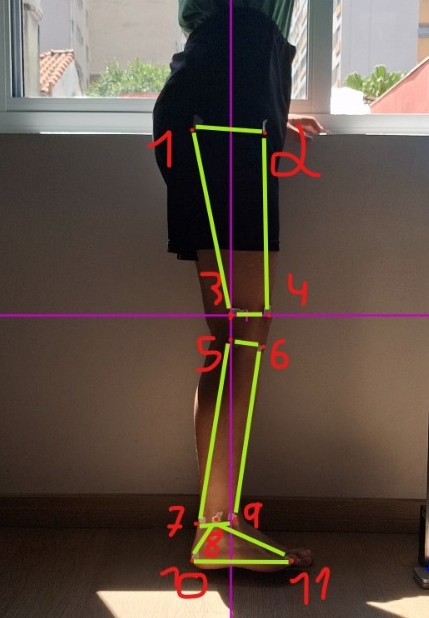
\includegraphics[width=0.36\textwidth]{figuras/rasc_p6_0.jpeg}
  \caption{Geometria adotada para a representação do membro inferior.}
  \label{fig:geometria}
\end{figure}

Na representação adotada, os pontos 1 e 2 estão localizados na região do quadril,
enquanto os pontos 3 e 4 estão posicionados na extremidade inferior da coxa, próxima à
região do joelho. Para a perna, os pontos 5 e 6 estão localizados imediatamente abaixo
do joelho, enquanto os pontos 7 e 9 estão posicionados aproximadamente na região do
tornozelo. O ponto 8 está localizado entre os pontos 7 e 9, contribuindo para a
representação da conexão entre a perna e o pé. Por fim, os pontos 10 e 11 correspondem
às extremidades inferiores da representação do pé.

A escolha de um mecanismo quadrilátero articulado para representar o movimento do
joelho está relacionada à necessidade de reproduzir adequadamente o movimento relativo
observado entre a coxa e a perna. Uma representação mais simples, na qual a coxa e a
perna fossem consideradas elementos rígidos conectados diretamente por uma única junta
de revolução, permitiria descrever apenas uma rotação da perna em torno de um centro
fixo. Nesse caso, os pontos pertencentes à perna descreveriam trajetórias circulares em
relação à coxa, o que constitui uma aproximação limitada do movimento do joelho.

O emprego de um quadrilátero articulado permite obter o movimento relativo entre a
coxa e a perna a partir da combinação das rotações de seus diferentes elos. Dessa
forma, o centro instantâneo do movimento relativo entre os segmentos (o polo $I_{13}$ da
\cref{sec:cadeia_fechada}) pode variar durante a movimentação, permitindo reproduzir
trajetórias mais complexas do que aquelas obtidas por uma única junta de revolução.
Essa característica é particularmente relevante para o problema proposto, uma vez que
o movimento relativo entre a coxa e a perna não pode ser rigorosamente representado
apenas por uma junta de rotação.

A representação do pé por meio de uma geometria triangular foi adotada de maneira
análoga, buscando preservar sua extensão e sua orientação em relação à perna. Uma
representação por um único elemento rígido poderia descrever apenas a distância entre
dois pontos, sem representar simultaneamente diferentes pontos de referência
associados ao pé. A geometria triangular fornece, portanto, uma representação rígida
simplificada da região, possibilitando acompanhar sua posição e orientação durante o
movimento.

Embora os pontos utilizados na aquisição experimental tenham sido definidos próximos
aos vértices das regiões utilizadas na representação geométrica, a localização das
articulações do mecanismo não está necessariamente restrita a esses pontos
experimentais. Articulações localizadas no interior das regiões correspondentes à coxa
e à perna também podem ser consideradas durante a síntese, desde que sejam compatíveis
com a geometria e com o movimento desejado.

\subsection{Aquisição experimental do movimento}\label{sec:aquisicao}

Após a definição da geometria, foram realizadas medições experimentais com o objetivo
de obter as posições dos pontos de interesse ao longo do movimento do membro inferior.
Para isso, um integrante do grupo realizou o movimento com a própria perna, e foi
registrada uma sequência de vídeo com o membro observado lateralmente.

Foram consideradas três configurações principais para caracterizar o movimento. A
configuração inicial corresponde à posição em pé, na qual a coxa, a perna e o pé se
encontram aproximadamente alinhados. A configuração intermediária corresponde a uma
flexão da perna de aproximadamente \SI{90}{\degree} em relação à coxa, mantendo-se a
posição da coxa. Por fim, a configuração final corresponde à condição de maior flexão
observada durante o experimento, na qual a perna se aproxima da coxa. A sequência de
configurações observada durante o movimento é apresentada na \cref{fig:sequencia}.

\begin{figure}[htbp]
  \centering
  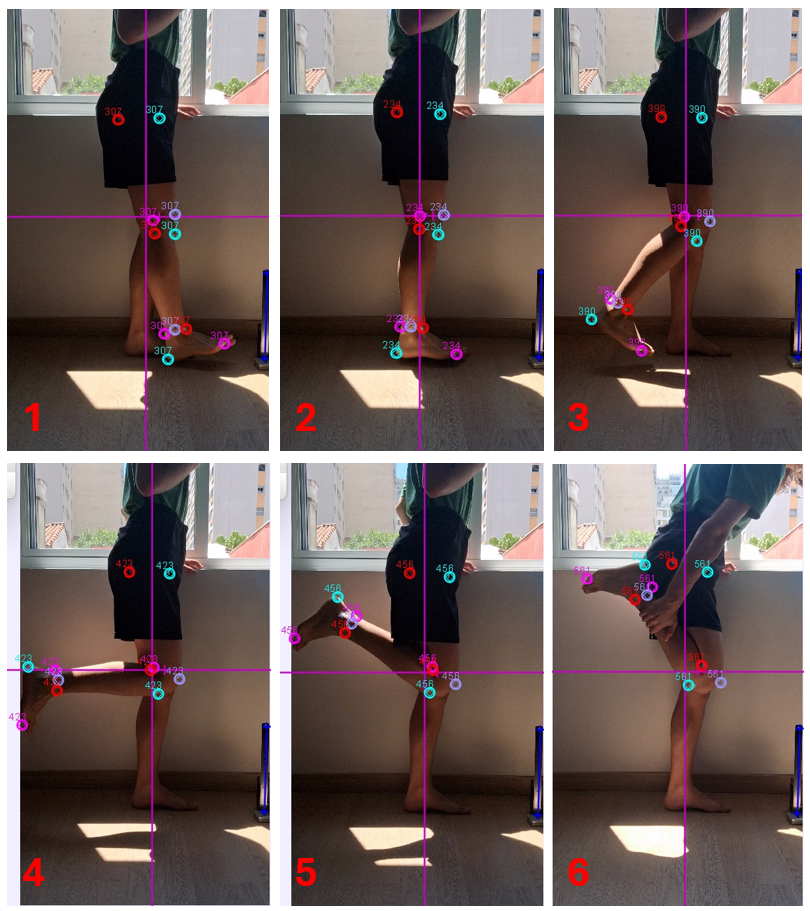
\includegraphics[width=0.62\textwidth]{figuras/rasc_p7_0.png}
  \caption{Sequência de configurações do membro inferior durante o movimento experimental.}
  \label{fig:sequencia}
\end{figure}

Para o processamento do vídeo foi empregado o software \emph{Tracker} \cite{tracker},
que permite acompanhar a posição de pontos específicos ao longo dos diferentes
\emph{frames} de uma gravação. Foram definidos pontos de referência próximos aos
vértices das regiões utilizadas na representação geométrica da coxa, da perna e do pé.
Esses pontos foram identificados e acompanhados individualmente ao longo do movimento,
permitindo obter suas coordenadas no plano da imagem em função do tempo. A numeração
dos pontos utilizada no rastreamento corresponde à geometria apresentada anteriormente
(\cref{fig:geometria}).

\begin{figure}[htbp]
  \centering
  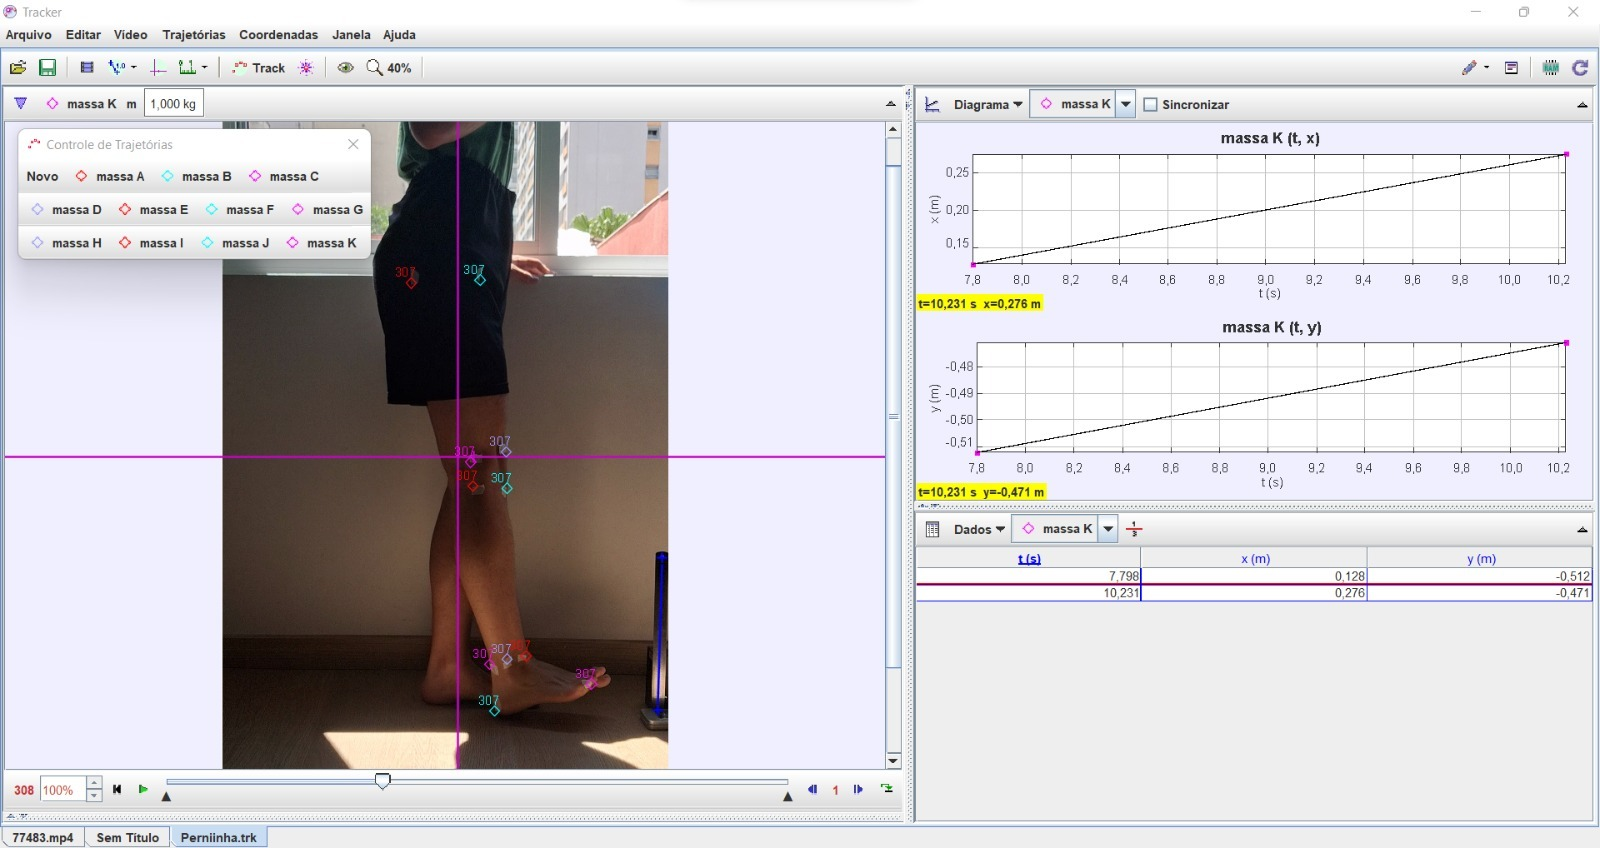
\includegraphics[width=\textwidth]{figuras/rasc_p8_0.jpeg}
  \caption{Rastreamento dos pontos do membro inferior e obtenção das posições no software \emph{Tracker}.}
  \label{fig:tracker}
\end{figure}

A partir do rastreamento, o \emph{Tracker} forneceu as coordenadas $x$ e $y$ dos pontos
acompanhados para os diferentes instantes analisados. Os valores obtidos correspondem,
portanto, às posições dos pontos no plano da imagem (base $im$, com a escala calibrada
em metros), e não diretamente aos comprimentos dos elos do mecanismo. O software também
permitiu visualizar graficamente a evolução temporal dessas coordenadas.

A planilha de dados obtida a partir do rastreamento contém as coordenadas dos onze
pontos para os \emph{frames} 234, 307, 390, 423, 456 e 561 (\cref{tab:tracker}, na
\cref{sec:anexos}). Para a análise do movimento, foram selecionados os \emph{frames}
307, 390, 423 e 456. O \emph{frame} 234 foi utilizado como referência durante a
identificação e numeração dos pontos, enquanto o \emph{frame} 561 foi desconsiderado,
pois corresponde a uma etapa do movimento em que houve auxílio manual para conduzir a
perna.

\subsection{Processamento dos dados e posições de precisão}\label{sec:processamento}

As coordenadas do \emph{Tracker} estão na base da imagem, e a coxa do voluntário também se
move ligeiramente entre os quadros. Como a síntese exige o movimento da perna
\emph{relativo} à coxa, os dados foram processados em três passos.

\paragraph{1º passo -- base da coxa em cada quadro.} A base $0$ tem origem no ponto médio
dos marcadores 3 e 4 (extremidade distal da coxa) e eixo $Y_0$ apontando para o ponto
médio dos marcadores 1 e 2 (quadril); $X_0$ aponta para a frente. Com
$\psi = \operatorname{atan2}(\Delta y, \Delta x) - \pi/2$, em que $(\Delta x, \Delta y)$ é o vetor
entre esses pontos médios na imagem,
\begin{equation}
  \Tm{im}{0} = \left[\begin{array}{c|c} \Rot{\psi}{z_0} & \tfrac12\big(\rv{im}{3} + \rv{im}{4}\big) \\ \hline \mathbf 0 & 1 \end{array}\right],
  \qquad
  \rv{0}{k} = \Rm{im}{0}^{\mathsf T}\Big(\rv{im}{k} - \tfrac12\big(\rv{im}{3} + \rv{im}{4}\big)\Big),
\end{equation}
em que se usou $\Rm{0}{im} = \Rm{im}{0}^{\mathsf T}$. O comprimento medido da coxa (entre os
pontos médios) variou entre \coxamin{} e \coxamax~mm nos quadros selecionados.

\paragraph{2º passo -- pose da perna.} A base $4$ é presa à perna e coincide com a base $0$
no quadro \frA{} (membro estendido). As coordenadas $\rv{4}{k}$ dos marcadores 5 a 9 são
as de $\rv{0}{k}$ nesse quadro, e a pose $\Tm{0}{4}^{(j)}$ de cada quadro $j$ é obtida pela
solução de Procrustes da \cref{sec:procrustes}. A flexão do joelho é $\varphi_j = -\alpha_j$.

\paragraph{3º passo -- tornozelo.} O ponto 8 (conexão perna--pé) tem, na base $4$,
$\rv{4}{P} = [\Px\ \ \Py]^{\mathsf T}$~mm, e sua posição em cada quadro é
$\big[\rv{0}{P};\,1\big] = \Tm{0}{4}^{(j)}\big[\rv{4}{P};\,1\big]$.

\begin{table}[htbp]
  \centering
  \caption{Poses da perna na base $0$ (coxa) obtidas das medições (mm). $\star$:
  posição de precisão; $\circ$: posição de verificação; $\dagger$: quadro não utilizado na
  síntese. Resíduo: erro quadrático médio do ajuste rígido dos marcadores 5 a 9.}
  \label{tab:poses}
  \begin{tabular}{lrrrrrr}
    \toprule
    Quadro & $\varphi$ (\si{\degree}) & ${}^0x_{O_4}$ & ${}^0y_{O_4}$ & ${}^0x_{P}$ & ${}^0y_{P}$ & Resíduo \\
    \midrule
    \tabelaposes
    \bottomrule
  \end{tabular}
\end{table}

\begin{figure}[htbp]
  \centering
  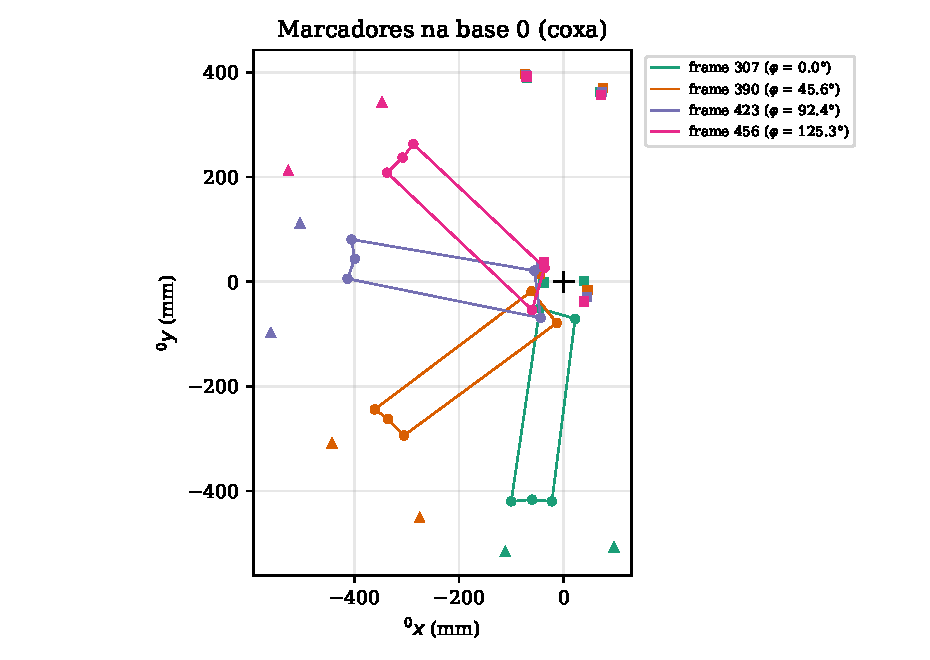
\includegraphics[width=0.85\textwidth]{figuras/p1_medicoes.pdf}
  \caption{Marcadores dos quadros selecionados escritos na base da coxa ($\square$: coxa,
  $\circ$: perna, $\triangle$: pé). A perna gira em torno da região do joelho enquanto a
  origem $O_4$ se desloca.}
  \label{fig:medicoes}
\end{figure}

Os quadros selecionados correspondem a flexões de \phiA, \phiB, \phiC{} e
\phiD\si{\degree} (\cref{tab:poses,fig:medicoes}), próximas das configurações inicial
(\SI{0}{\degree}), intermediárias (\SI{45}{\degree} e \SI{90}{\degree}) e de máxima
flexão. O resíduo do ajuste rígido, entre \resmin{} e \resmax~mm, reflete os artefatos de
pele e a imprecisão da marcação manual, e cresce com a flexão, quando os marcadores se
deslocam mais sobre a pele. Nota-se também que a origem $O_4$ se desloca cerca de
\SI{57}{mm} durante o movimento: esse é justamente o efeito que uma junta de revolução
simples não reproduz e que motiva o uso do quadrilátero.

\paragraph{Escolha das posições de precisão.} Dispondo de quatro posições medidas, três
são usadas como posições de precisão na síntese e a quarta é usada para verificação.
Foram testadas as três combinações que incluem a extensão completa (\cref{tab:combos});
adotou-se a que resultou no menor custo \eqref{eq:custo}: quadros \precA, \precB{} e \precC{}
como posições de precisão e o quadro \cheque{} ($\varphi = \phicheque\si{\degree}$) como
verificação.

\begin{table}[htbp]
  \centering
  \caption{Combinações de posições de precisão testadas.}
  \label{tab:combos}
  \begin{tabular}{lccc}
    \toprule
    Precisão (quadros) & Verificação & Erro na verificação (mm) & $\mu_{\min}$ (\si{\degree}) \\
    \midrule
    \tabelacombos
    \bottomrule
  \end{tabular}
\end{table}

\subsection{Escolha dos pivôs móveis}\label{sec:escolha}

Com três posições, qualquer escolha de $\big(\rv{4}{Q}, \rv{4}{N}\big)$ gera, por
\eqref{eq:circuncentro}, um mecanismo que passa exatamente pelas posições de precisão.
As duas escolhas livres por díade são usadas para aproximar também a posição de
verificação e para impor requisitos de projeto. Para cada candidato, o mecanismo é
montado pela equação de fechamento \eqref{eq:fechamento} e o erro no tornozelo é
\begin{equation}
  e_j = \Big\lVert \rv{0}{P}^{\,\mathrm{mec}}(\varphi_j) - \rv{0}{P}^{\,\mathrm{med}}(\varphi_j) \Big\rVert ,
\end{equation}
comparando mecanismo e medição para a mesma orientação da perna. Minimiza-se
\begin{equation}
  J\big(\rv{4}{Q},\rv{4}{N}\big) = e_{\mathrm{verificação}} + \text{penalidades},
  \label{eq:custo}
\end{equation}
em que as penalidades impõem: $\mu \ge \SI{30}{\degree}$ em toda a faixa; pivôs fixos na
região do joelho ($|{}^0x| \le \SI{60}{mm}$, $\SI{-40}{mm} \le {}^0y \le \SI{60}{mm}$);
elos entre \SI{20}{mm} e \SI{120}{mm}; e montagem contínua (mesmo ramo) de
\SI{0}{\degree} até a flexão máxima medida -- o que elimina os defeitos de ramo e de ordem.
A busca combina amostragem aleatória (3000 candidatos) e refinamento por Nelder--Mead.

\section{Parte I -- Resultados da síntese}\label{cap:resultados1}

\subsection{Mecanismo sintetizado}

A otimização convergiu para os pivôs da \cref{tab:pivos}. Os pivôs fixos $C$ e $L$ ficam
logo abaixo dos marcadores 3 e 4, na região da articulação do joelho, e os pivôs
móveis $Q$ e $N$ ficam sobre a perna.

\begin{table}[htbp]
  \centering
  \caption{Resultado da síntese dimensional com as medições do grupo (mm).}
  \label{tab:pivos}
  \begin{tabular}{lll}
    \toprule
    Articulação & Elo & Coordenadas \\
    \midrule
    $C$ & coxa (fixo) & $\rv{0}{C} = [\Cx\ \ \Cy]^{\mathsf T}$ \\
    $L$ & coxa (fixo) & $\rv{0}{L} = [\Lx\ \ \Ly]^{\mathsf T}$ \\
    $Q$ & perna (móvel) & $\rv{4}{Q} = [\Qx\ \ \Qy]^{\mathsf T}$ \\
    $N$ & perna (móvel) & $\rv{4}{N} = [\Nx\ \ \Ny]^{\mathsf T}$ \\
    \midrule
    \multicolumn{3}{l}{Comprimentos: $\ell_0 = \overline{CL} = \rCL$, $\ell_1 = \overline{CQ} = \rCQ$, $\ell_2 = \overline{QN} = \rQN$, $\ell_3 = \overline{LN} = \rLN$} \\
    \bottomrule
  \end{tabular}
\end{table}

\paragraph{Grashof.} Com $s=\grashofs$, $p=\grashofp$, $q=\grashofq$ e $l=\grashofl$~mm,
$s+l=\grashofsl \grashofsinal p+q=\grashofpq$: o mecanismo \grashof{} a condição
\eqref{eq:grashof}. A simulação de montagem confirma que ele percorre continuamente a
faixa de \SI{0}{\degree} a \phimax\si{\degree} sem atingir pontos mortos, com $\mu$ entre
\mumin\si{\degree} e \mumax\si{\degree} (\cref{fig:erro}).

\paragraph{Precisão.} Nas três posições de precisão o erro é nulo (a menos da tolerância
numérica), como esperado. Na posição de verificação (quadro \cheque,
$\varphi = \phicheque\si{\degree}$), o erro no tornozelo é de \errcheque~mm, inferior ao
resíduo das próprias medições (\resmin{} a \resmax~mm). O mecanismo reproduz, portanto,
o movimento medido dentro da incerteza experimental. A \cref{fig:mecanismo} mostra o
mecanismo nas quatro posições medidas, a centroide (trajetória do polo $I_{13}$) e a
trajetória do tornozelo.

\begin{figure}[htbp]
  \centering
  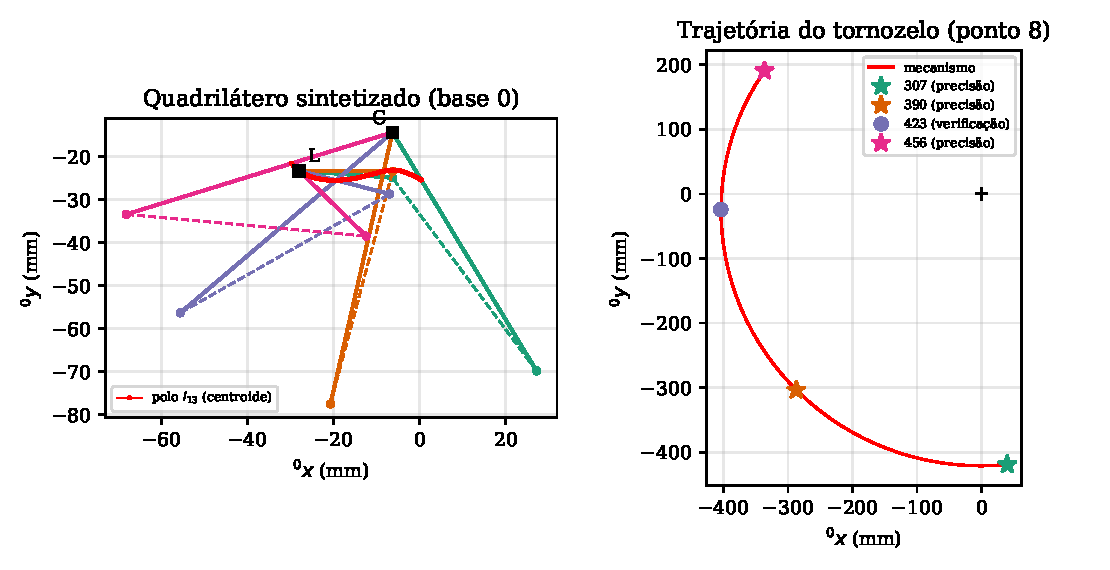
\includegraphics[width=\textwidth]{figuras/p1_mecanismo.pdf}
  \caption{Esquerda: quadrilátero sintetizado nas quatro posições medidas (tracejado:
  acoplador $QN$) e centroide. Direita: trajetória do tornozelo gerada pelo mecanismo e
  posições medidas.}
  \label{fig:mecanismo}
\end{figure}

\begin{figure}[htbp]
  \centering
  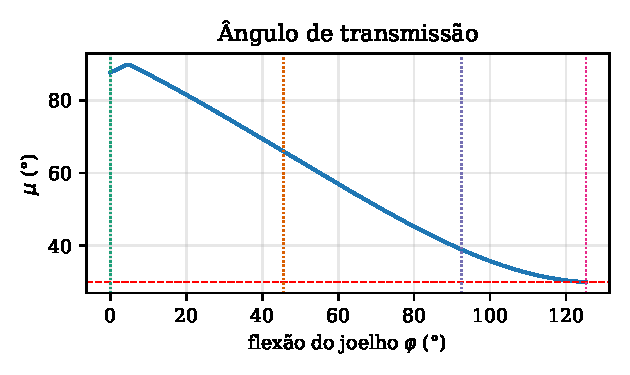
\includegraphics[width=0.6\textwidth]{figuras/p1_erro_mu.pdf}
  \caption{Ângulo de transmissão em função da flexão (linhas verticais: posições medidas).}
  \label{fig:erro}
\end{figure}

\subsection{Discussão}

O ângulo de transmissão mínimo ocorre na flexão máxima e fica no limite de
\SI{30}{\degree} imposto na otimização, o que indica que a restrição está ativa: exigir
um $\mu$ maior aumentaria o erro na posição de verificação. O polo parte de
$(\ciOx;\ \ciOy)$~mm na extensão e migra posteriormente até $(\ciFx;\ \ciFy)$~mm na
flexão máxima, comportamento qualitativamente semelhante à centroide em ``J'' descrita
por \textcite{oconnor1989}. Como as medições têm resíduo de até \resmax~mm, o
refinamento natural do projeto é usar mais quadros do vídeo em uma síntese por mínimos
quadrados. Para uma prótese transfemoral real, recomenda-se ainda verificar a posição
do polo em extensão em relação à linha trocânter--joelho--tornozelo, da qual depende a
estabilidade voluntária na fase de apoio \cite{radcliffe1994}.

\subsection{Maquete}\label{cap:maquete}

A maquete, em escala 1:1, permite avaliar qualitativamente o funcionamento do
mecanismo. O programa gera um gabarito em A4 (\texttt{figuras/p1\_gabarito\_maquete.pdf},
\cref{fig:gabarito}) com a posição exata dos furos.

\begin{itemize}
  \item \textbf{Material}: MDF ou acrílico de \SI{3}{mm} (corte a laser) para as placas da
  coxa e da perna; os elos $CQ$ e $LN$ em acrílico de \SI{3}{mm} ou alumínio em chapa de
  \SI{2}{mm}.
  \item \textbf{Articulações}: parafusos M4 com arruelas de náilon e porcas
  autotravantes (ou rebites de repuxo de \SI{4}{mm}), furos de \SI{4,2}{mm}. Os elos
  $CQ$ e $LN$ devem ficar em planos diferentes (um de cada lado das placas) para que
  não colidam quando se cruzam.
  \item \textbf{Segmentos}: a placa da coxa prolonga-se até o quadril (cerca de \SI{375}{mm},
  comprimento medido) e a da perna até o tornozelo (ponto 8), com o pé triangular
  (pontos 8, 10 e 11) fixado rigidamente.
\end{itemize}

\noindent\textbf{Ensaios qualitativos sugeridos}: (1) verificar a faixa de movimento de
\SI{0}{\degree} a \phimax\si{\degree}; (2) comparar lado a lado com o movimento filmado,
fotografando a maquete nas mesmas flexões dos quadros da \cref{tab:poses}; (3) marcar o polo (intersecção de $CQ$ e $LN$) com uma linha
esticada e observar a migração da centroide; (4) aplicar carga vertical com o joelho
estendido e observar a tendência de flexão.

\begin{figure}[htbp]
  \centering
  \fbox{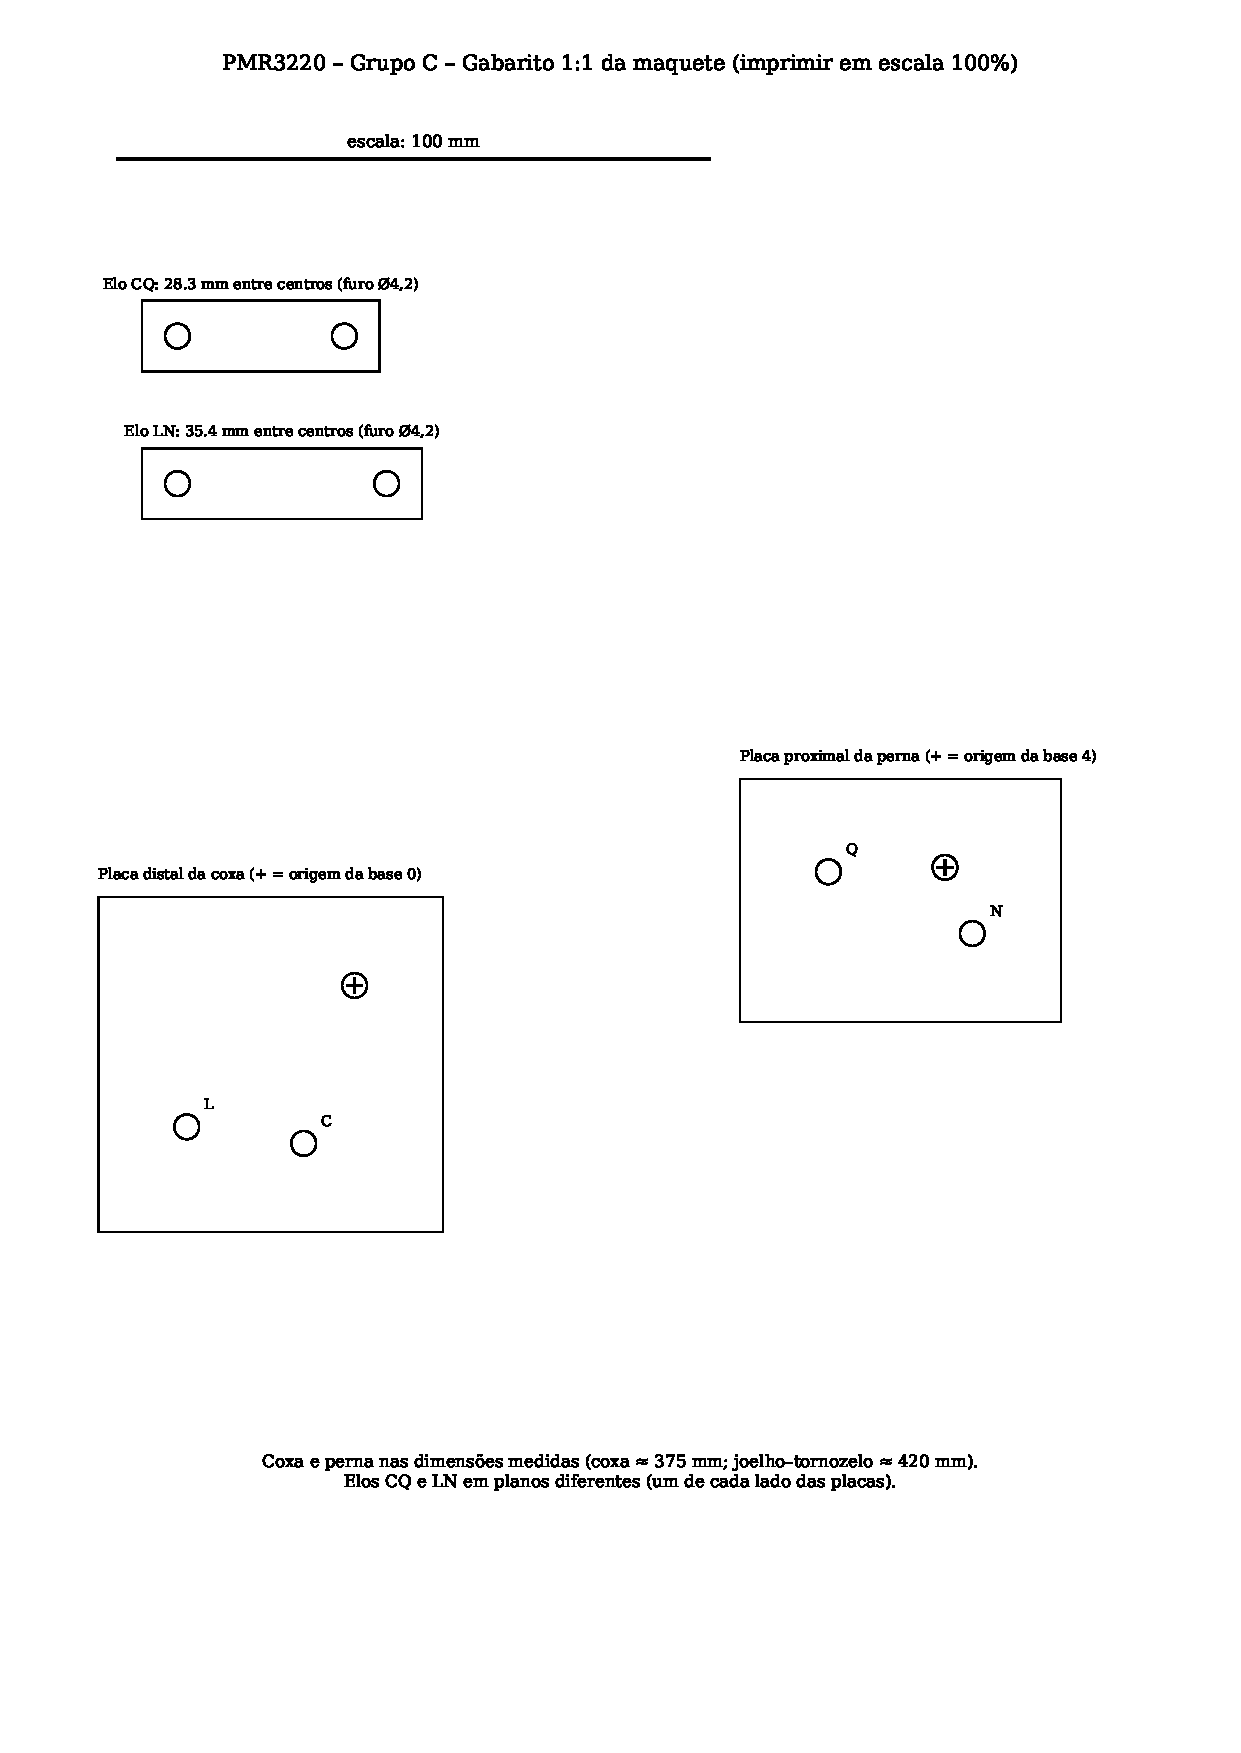
\includegraphics[width=0.55\textwidth]{figuras/p1_gabarito_maquete.pdf}}
  \caption{Gabarito da maquete (imprimir em escala 100\%).}
  \label{fig:gabarito}
\end{figure}

\section{Parte II -- Modelagem cinemática}\label{cap:cinematica}

Nesta parte, analisa-se uma órtese para um indivíduo de \SIrange{60}{80}{kg} cuja
capacidade motora do membro inferior foi comprometida (por exemplo, por um AVC ou por
lesão causada por esforço físico intenso). A análise cinemática é feita a partir das
configurações dadas no enunciado (\cref{fig:enunciado}b), usando as mesmas ferramentas
do método matricial empregadas na Parte~I.

\subsection{Hipóteses}

\begin{hipotese}
O movimento ocorre no plano sagital, e o tronco está imóvel; o quadril $D$ é, portanto,
um ponto fixo (base do manipulador).
\end{hipotese}
\begin{hipotese}
O joelho da órtese é modelado como junta de revolução em $O$ (o joelho policêntrico da
Parte~I pode ser incorporado depois, com efeito pequeno nos torques).
\end{hipotese}
\begin{hipotese}
O pé e a perna formam um único corpo rígido, com o pé $PR$ perpendicular à perna $OP$.
O enunciado diz ``pé e coxa'', mas a \cref{fig:enunciado}b mostra que $PR \perp OP$ nas
três configurações; conclui-se tratar-se de um erro de digitação.
\end{hipotese}
\begin{hipotese}
A musculatura está inativa: os torques são fornecidos inteiramente pelos atuadores do
quadril (fixo no tronco) e do joelho (estator fixo na coxa). Não há contato do pé com o
solo durante o ciclo, e o atrito nas juntas é desprezado.
\end{hipotese}
\begin{hipotese}
$\overline{DO} = \ell_1 = \SI{0,40}{m}$, $\overline{OP} = \ell_2 = \SI{0,45}{m}$,
$\overline{PR} = \ell_3 = \SI{0,25}{m}$ (enunciado).
\end{hipotese}

\subsection{Bases e cinemática direta (cadeia aberta RR)}

O membro com a órtese é uma cadeia aberta de duas juntas de revolução, análoga ao
mecanismo RR do método matricial. As bases são (\cref{fig:modelo}):
\begin{itemize}
  \item base $0$ (fixa, tronco): origem em $D$, $X_0$ horizontal para a frente, $Y_0$
  vertical para cima;
  \item base $1$ (coxa): origem em $D$, $X_1$ ao longo de $DO$; $\theta_1$ é o ângulo de $X_0$
  para $X_1$ (junta do quadril);
  \item base $2$ (perna + pé): origem em $O$, $X_2$ ao longo de $OP$ e $Y_2$ no sentido $PR$;
  $\theta_2$ é o ângulo \emph{relativo} de $X_1$ para $X_2$ (junta do joelho).
\end{itemize}
A orientação absoluta da perna é, portanto, $\theta_1 + \theta_2$, e as coordenadas
generalizadas são $\mathbf q = [\theta_1\ \ \theta_2]^{\mathsf T}$. As transformações homogêneas são
\begin{equation}
  \Tm{0}{1} = \left[\begin{array}{c|c} \Rm{0}{1} & \rv{0}{O_1} \\ \hline \mathbf 0 & 1 \end{array}\right]
            = \left[\begin{array}{cc|c} c_1 & -s_1 & 0\\ s_1 & c_1 & 0\\ \hline 0 & 0 & 1\end{array}\right],
  \qquad
  \Tm{1}{2} = \left[\begin{array}{c|c} \Rm{1}{2} & \rv{1}{O_2} \\ \hline \mathbf 0 & 1 \end{array}\right]
            = \left[\begin{array}{cc|c} c_2 & -s_2 & \ell_1\\ s_2 & c_2 & 0\\ \hline 0 & 0 & 1\end{array}\right],
\end{equation}
com $\Rm{0}{1} = \Rot{\theta_1}{z_1}$ e $\Rm{1}{2} = \Rot{\theta_2}{z_2}$. Os pontos de interesse têm
coordenadas constantes nas bases dos seus elos: $\rv{1}{O} = [\ell_1\ \ 0]^{\mathsf T}$,
$\rv{2}{P} = [\ell_2\ \ 0]^{\mathsf T}$ e $\rv{2}{R} = [\ell_2\ \ \ell_3]^{\mathsf T}$. Assim,
\begin{align}
  \hmg{\rv{0}{P}} &= \Tm{0}{1}\,\Tm{1}{2}\hmg{\rv{2}{P}}
   = \begin{bmatrix} c_1 & -s_1 & 0\\ s_1 & c_1 & 0\\ 0 & 0 & 1\end{bmatrix}
     \begin{bmatrix} \ell_2 c_2 + \ell_1\\ \ell_2 s_2 \\ 1\end{bmatrix}
   = \begin{bmatrix} \ell_1 c_1 + \ell_2 c_{12}\\ \ell_1 s_1 + \ell_2 s_{12} \\ 1\end{bmatrix},
  \label{eq:posP}\\
  \hmg{\rv{0}{R}} &= \Tm{0}{1}\,\Tm{1}{2}\hmg{\rv{2}{R}}
   = \begin{bmatrix} \ell_1 c_1 + \ell_2 c_{12} - \ell_3 s_{12}\\ \ell_1 s_1 + \ell_2 s_{12} + \ell_3 c_{12} \\ 1\end{bmatrix},
\end{align}
e $\hmg{\rv{0}{O}} = \Tm{0}{1}\hmg{\rv{1}{O}} = [\ell_1 c_1\ \ \ell_1 s_1\ \ 1]^{\mathsf T}$.

\paragraph{Velocidades e acelerações.} Derivando \eqref{eq:posP} no tempo, com $\rv{2}{P}$
constante,
\begin{align}
  \hoz{\rvd{0}{P}} &= \big(\Tmd{0}{1}\,\Tm{1}{2} + \Tm{0}{1}\,\Tmd{1}{2}\big)\hmg{\rv{2}{P}},\\
  \hoz{\rvdd{0}{P}} &= \big(\Tmdd{0}{1}\,\Tm{1}{2} + 2\,\Tmd{0}{1}\,\Tmd{1}{2} + \Tm{0}{1}\,\Tmdd{1}{2}\big)\hmg{\rv{2}{P}},
\end{align}
em que
\begin{equation}
  \Tmd{0}{1} = \begin{bmatrix} -s_1 & -c_1 & 0\\ c_1 & -s_1 & 0\\ 0 & 0 & 0\end{bmatrix}\dot\theta_1,
  \qquad
  \Tmdd{0}{1} = \begin{bmatrix} -c_1 & s_1 & 0\\ -s_1 & -c_1 & 0\\ 0 & 0 & 0\end{bmatrix}\dot\theta_1^2
              + \begin{bmatrix} -s_1 & -c_1 & 0\\ c_1 & -s_1 & 0\\ 0 & 0 & 0\end{bmatrix}\ddot\theta_1,
\end{equation}
e analogamente para $\Tmd{1}{2}$ e $\Tmdd{1}{2}$ com $\theta_2$ (a translação $\ell_1$ é constante e
some na derivada). Efetuando os produtos,
\begin{equation}
  \rvd{0}{P} = \begin{bmatrix} -\ell_1 s_1 - \ell_2 s_{12} & -\ell_2 s_{12}\\ \ell_1 c_1 + \ell_2 c_{12} & \ell_2 c_{12}\end{bmatrix}
               \begin{bmatrix}\dot\theta_1\\ \dot\theta_2\end{bmatrix} = \Jm{P}\,\dot{\mathbf q},
\end{equation}
em que $\Jm{P}$ é a matriz jacobiana do ponto $P$. As velocidades e acelerações angulares
dos elos são
\begin{equation}
  {}^0\boldsymbol\omega_1 = \dot\theta_1\,\mathbf k_0,\quad
  {}^0\boldsymbol\omega_2 = (\dot\theta_1+\dot\theta_2)\,\mathbf k_0,\quad
  {}^0\dot{\boldsymbol\omega}_1 = \ddot\theta_1\,\mathbf k_0,\quad
  {}^0\dot{\boldsymbol\omega}_2 = (\ddot\theta_1+\ddot\theta_2)\,\mathbf k_0 .
\end{equation}

\begin{figure}[htbp]
  \centering
  \begin{tikzpicture}[scale=7.5, >=Stealth]
    \coordinate (D) at (0,0);
    \coordinate (O) at ({0.40*cos(-35)},{0.40*sin(-35)});
    \coordinate (P) at ($(O)+({0.45*cos(-120)},{0.45*sin(-120)})$);
    \coordinate (R) at ($(P)+({0.25*cos(-30)},{0.25*sin(-30)})$);
    \fill[pattern=north east lines] (-0.1,0.0) rectangle (-0.04,0.06);
    \draw[very thick] (D) -- node[below left, pos=0.7] {$\ell_1$} (O) -- node[left] {$\ell_2$} (P) -- node[below left] {$\ell_3$} (R);
    \foreach \p in {D,O} \draw[fill=white] (\p) circle (0.018);
    \foreach \p in {P,R} \fill (\p) circle (0.012);
    \node[left] at ($(D)+(-0.1,0)$) {$D$};
    \node[above right] at ($(O)+(0.01,0.01)$) {$O$};
    \node[left] at (P) {$P$};
    \node[right] at (R) {$R$};
    % base 0
    \draw[->,thick] (D) -- (0.25,0) coordinate (Z0) node[right] {$X_0$};
    \draw[->,thick] (D) -- (0,0.15) node[above] {$Y_0$};
    % base 1
    \draw[->,teal,thick] (D) -- ($(D)!0.35!(O)$) node[below left] {$X_1$};
    \pic[draw,<-,blue,"$\theta_1$",angle radius=1.6cm,angle eccentricity=1.2] {angle=O--D--Z0};
    % base 2
    \draw[dashed,blue] (O) -- ($(O)+({0.25*cos(-35)},{0.25*sin(-35)})$) coordinate (Oe);
    \draw[->,teal,thick] (O) -- ($(O)!0.3!(P)$) node[left] {$X_2$};
    \draw[->,teal,thick] (O) -- ($(O)+({0.15*cos(-30)},{0.15*sin(-30)})$) node[right] {$Y_2$};
    \pic[draw,<-,blue,"$\theta_2$",angle radius=1.3cm,angle eccentricity=1.2] {angle=P--O--Oe};
    \draw[->] (-0.25,-0.6) -- (-0.25,-0.7) node[right] {$\mathbf g$};
  \end{tikzpicture}
  \caption{Cadeia aberta RR da órtese: bases $0$ (fixa), $1$ (coxa) e $2$ (perna + pé).
  $\theta_1$ é medido de $X_0$ para $X_1$ e $\theta_2$, de $X_1$ para $X_2$ (na figura, ambos
  negativos, isto é, no sentido horário).}
  \label{fig:modelo}
\end{figure}

\subsection{Configurações extremas}

Os ângulos foram lidos da \cref{fig:enunciado}b. Na configuração final~I, a coxa está a
\SI{280,13}{\degree} e o ângulo interno do joelho é \SI{60}{\degree}; na final~II, a coxa está
a \SI{10,07}{\degree} e o ângulo interno é \SI{70,1}{\degree}. Como o ângulo interno entre
$\overrightarrow{OD}$ e $\overrightarrow{OP}$ é $\SI{180}{\degree} - |\theta_2|$, com a flexão
do joelho no sentido horário ($\theta_2<0$):

\begin{table}[htbp]
  \centering
  \caption{Configurações extremas do ciclo.}
  \label{tab:config}
  \begin{tabular}{lrrrl}
    \toprule
    Configuração & $\theta_1$ (\si{\degree}) & $\theta_2$ (\si{\degree}) & $\theta_1+\theta_2$ (\si{\degree}) & Movimento \\
    \midrule
    inicial  & $-90{,}00$ & $0{,}00$ & $-90{,}00$ & em pé, joelho estendido \\
    final I  & $-79{,}87$ & $-120{,}00$ & $-199{,}87$ & flexão do joelho (``chute para trás'') \\
    final II & $10{,}07$ & $-109{,}90$ & $-99{,}83$ & flexão de quadril e joelho (``marcha alta'') \\
    \bottomrule
  \end{tabular}
\end{table}

A consistência foi conferida com a direção do pé ($Y_2$), $\theta_1+\theta_2 + \SI{90}{\degree}$, que vale
\SI{0}{\degree}, \SI{-109,9}{\degree} e \SI{-9,8}{\degree} nas três configurações, de acordo com os
segmentos $PR$ da figura.

\subsection{Interpolação polinomial de 5º grau}

Para cada coordenada generalizada $q\in\{\theta_1,\theta_2\}$, adota-se
$q(t) = \sum_{k=0}^{5} a_k t^k$, cujos seis coeficientes são determinados pelas condições
de contorno de posição, velocidade e aceleração no início e no fim do trecho:
\begin{equation}
  q(0)=q_0,\ \dot q(0)=0,\ \ddot q(0)=0,\qquad q(T)=q_f,\ \dot q(T)=0,\ \ddot q(T)=0 .
\end{equation}
As três primeiras fornecem $a_0 = q_0$, $a_1 = a_2 = 0$; as restantes formam o sistema
\begin{equation}
  \begin{bmatrix} T^3 & T^4 & T^5\\ 3T^2 & 4T^3 & 5T^4 \\ 6T & 12T^2 & 20T^3 \end{bmatrix}
  \begin{bmatrix} a_3\\ a_4\\ a_5\end{bmatrix}
  = \begin{bmatrix} \Delta q\\ 0\\ 0\end{bmatrix}
  \;\Rightarrow\;
  a_3 = \frac{10\,\Delta q}{T^3},\ a_4 = -\frac{15\,\Delta q}{T^4},\ a_5 = \frac{6\,\Delta q}{T^5},
\end{equation}
com $\Delta q = q_f - q_0$. Com o tempo normalizado $\tau = t/T\in[0,1]$:
\begin{align}
  q(t) &= q_0 + \Delta q\,\big(10\tau^3 - 15\tau^4 + 6\tau^5\big), \label{eq:quint}\\
  \dot q(t) &= \frac{\Delta q}{T}\,30\tau^2\big(1-\tau\big)^2, \\
  \ddot q(t) &= \frac{\Delta q}{T^2}\,60\tau\big(1-\tau\big)\big(1-2\tau\big).
\end{align}
Os valores extremos são obtidos anulando as derivadas. A velocidade é máxima onde
$\ddot q = 0$ no interior do intervalo, isto é, em $\tau = \tfrac12$, e vale
$30\cdot\tfrac14\cdot\tfrac14 = \tfrac{15}{8}$ vezes $\Delta q/T$. A aceleração é extrema onde
$\mathrm d\ddot q/\mathrm d\tau \propto 1 - 6\tau + 6\tau^2 = 0$, ou seja,
$\tau = \tfrac12 \mp \tfrac{\sqrt3}{6}$; nesses pontos $\tau(1-\tau) = \tfrac16$ e
$1 - 2\tau = \pm\tfrac{\sqrt3}{3}$, de modo que
\begin{equation}
  \dot q_{\max} = \frac{15}{8}\frac{\Delta q}{T}\ \ (\tau=\tfrac12),\qquad
  |\ddot q|_{\max} = 60\cdot\frac16\cdot\frac{\sqrt3}{3}\,\frac{|\Delta q|}{T^2} = \frac{10\sqrt3}{3}\frac{|\Delta q|}{T^2}\ \ \Big(\tau = \tfrac12 \mp \tfrac{\sqrt3}{6}\Big).
  \label{eq:picos}
\end{equation}
\emph{Exemplo:} para o joelho na configuração final~I, $\Delta q = \SI{120}{\degree}$ e $T = \SI{2}{s}$
fornecem $\dot q_{\max} = \tfrac{15}{8}\cdot\tfrac{120}{2} = \SI{112,5}{\degree\per\s}$ e
$|\ddot q|_{\max} = 5{,}774\cdot\tfrac{120}{4} = \SI{173,2}{\degree\per\s\squared}$.
A quíntica garante aceleração contínua e nula nas extremidades, portanto torque sem
descontinuidades e sem excitação de modos flexíveis -- vantagem sobre o polinômio
cúbico, cuja aceleração salta no início e no fim \cite{craig2005,siciliano2009}.

\paragraph{Ciclo completo e escolha de $T$.} O ciclo é composto pela ida (inicial
$\to$ final) em $[0,T]$ e pelo retorno em $[T, 2T]$, também por quíntica. Como o
polinômio normalizado $s(\tau)$ satisfaz $s(1-\tau) = 1 - s(\tau)$, o retorno é o espelho
temporal da ida, $q(t) = q(2T-t)$: as velocidades trocam de sinal, e as acelerações se
repetem. Como os termos de velocidade da dinâmica são quadráticos, os torques também
são simétricos em relação a $t=T$. Adotou-se $T = \SI{2}{s}$ por trecho (ciclo de
\SI{4}{s}), o que, por \eqref{eq:picos}, resulta em velocidades máximas de
\SIrange{94}{113}{\degree\per\s}: valores inferiores aos da marcha normal (até cerca de
\SI{350}{\degree\per\s} no joelho, \cite{winter2009}) e adequados à reabilitação de um
indivíduo com musculatura inativa. A sensibilidade a $T$ é analisada no
\cref{cap:resultados2}.

\section{Parte II -- Parâmetros de massa e inércia}\label{cap:parametros}

\subsection{Dados antropométricos}

Utilizaram-se as tabelas de \textcite{winter2009}, baseadas em \textcite{drillis1964}
e amplamente usadas em análise de marcha. As massas são frações da massa corporal $M$;
as posições do centro de massa (CM) e o raio de giração baricêntrico $\rho$ são frações
do comprimento do segmento (\cref{tab:winter}). A estatura correspondente a
$\ell_1 = \SI{0,40}{m}$ é $H = \ell_1/0{,}245 \approx \SI{1,63}{m}$ \cite{drillis1964}.

\begin{table}[htbp]
  \centering
  \caption{Parâmetros segmentares \cite{winter2009}.}
  \label{tab:winter}
  \small
  \begin{tabular}{lcccc}
    \toprule
    Segmento & $m/M$ & $x_{\mathrm{CM}}/L$ (a partir de) & $\rho_{\mathrm{CM}}/L$ & Comprimento $L$ \\
    \midrule
    Coxa  & 0,100  & 0,433 (quadril)   & 0,323 & $\ell_1 = \SI{0,40}{m}$ \\
    Perna & 0,0465 & 0,433 (joelho)    & 0,302 & $\ell_2 = \SI{0,45}{m}$ \\
    Pé    & 0,0145 & 0,50 (ao longo de $PR$) & 0,475 & $\ell_3 = \SI{0,25}{m}$ \\
    \bottomrule
  \end{tabular}
\end{table}

Para cada segmento, o momento de inércia baricêntrico é $I = m(\rho\,L)^2$. Para
$M = \SI{80}{kg}$, por exemplo, a coxa tem $m = 0{,}100\cdot 80 = \SI{8,0}{kg}$, CM a
$0{,}433\cdot 0{,}40 = \SI{0,173}{m}$ do quadril e $I = 8{,}0\,(0{,}323\cdot 0{,}40)^2 = \SI{0,134}{kg.m^2}$;
a perna tem \SI{3,72}{kg} e o pé, \SI{1,16}{kg}.

\subsection{Seleção de materiais da órtese}

A órtese é do tipo joelho--tornozelo--pé (KAFO) ativa, com hastes laterais e mediais,
braçadeiras e palmilha. Os materiais foram selecionados em referências de elementos de
máquinas e de materiais \cite{shigley2015,asm1990,callister2018} e de órteses
\cite{edelstein2011} (\cref{tab:materiais}).

\begin{table}[htbp]
  \centering
  \caption{Propriedades dos materiais selecionados.}
  \label{tab:materiais}
  \small
  \setlength{\tabcolsep}{4pt}
  \begin{tabular}{p{3.0cm}cccccp{2.6cm}}
    \toprule
    Material & $\rho$ (\si{kg/m^3}) & $E$ (GPa) & $S_y$ (MPa) & $S_u$ (MPa) & $S_e$ (MPa) & Uso \\
    \midrule
    Al 6061-T6 & 2700 & 68,9 & 276 & 310 & 96,5\textsuperscript{a} & hastes, estribo \\
    Aço inox AISI 304 (recozido) & 8000 & 193 & 215 & 505 & -- & eixo e mancais do joelho \\
    Polipropileno copolímero & 905 & 1,3 & 28 & 32 & -- & braçadeiras e palmilha \\
    Compósito carbono/epóxi\textsuperscript{b} & 1550 & 70 & -- & 600 & -- & alternativa às hastes \\
    \bottomrule
  \end{tabular}\\[2pt]
  \footnotesize \textsuperscript{a}Resistência à fadiga para $5\times10^8$ ciclos \cite{asm1990}.
  \textsuperscript{b}Tecido bidirecional, laminado quase-isotrópico (valores típicos).
\end{table}

O alumínio 6061-T6 alia boa relação resistência/massa (cerca de 1/3 da densidade do aço),
usinabilidade e soldabilidade, e é o padrão em hastes de órteses; o polipropileno é
termoformável sobre o molde do membro; o aço inox é usado nas partes sujeitas a
desgaste e contato. As hastes têm seção retangular de \qtyproduct{20 x 5}{mm} (\SI{20}{mm} no plano
sagital). A \cref{tab:ortese} lista as massas dos componentes, calculadas a partir da
geometria e da densidade; a massa total da órtese é de \massaOrtese~kg, dentro da faixa
de KAFOs motorizadas.

\begin{table}[htbp]
  \centering
  \caption{Componentes da órtese: massa e posição do CM no referencial do elo (m). Elo~1:
  origem em $D$, $x$ ao longo de $DO$. Elo~2: origem em $O$, $x$ ao longo de $OP$, $y$ no
  sentido $PR$.}
  \label{tab:ortese}
  \small
  \begin{tabular}{llrl}
    \toprule
    Elo & Componente & $m$ (kg) & CM $(x;\,y)$ \\
    \midrule
    \tabelaortese
    \bottomrule
  \end{tabular}
\end{table}

O atuador do quadril está fixo ao tronco (cinto pélvico) e não pertence a nenhum elo
móvel; o do joelho tem o estator fixo na coxa.

\subsection{Parâmetros equivalentes dos elos}

Cada elo $i$ é um corpo rígido composto. Para componentes de massa $m_k$, centro de massa
$\rv{i}{k}$ (escrito na base do próprio elo, onde é constante) e inércia própria $I_k$:
\begin{equation}
  m_i = \sum_k m_k,\qquad
  \rv{i}{G_i} = \frac{1}{m_i}\sum_k m_k\,\rv{i}{k},\qquad
  I_i = \sum_k \Big[I_k + m_k \big(\rv{i}{k} - \rv{i}{G_i}\big)^{\mathsf T}\big(\rv{i}{k} - \rv{i}{G_i}\big)\Big] \quad\text{(Steiner)}.
\end{equation}
Os centros de massa resultantes são $\rv{1}{G_1} = [a_1\ \ 0]^{\mathsf T}$ (sobre o eixo $X_1$) e
$\rv{2}{G_2} = [b_x\ \ b_y]^{\mathsf T}$: o elo~2 tem o CM fora do eixo $X_2$, deslocado no sentido do pé.

\begin{table}[htbp]
  \centering
  \caption{Parâmetros equivalentes dos elos (membro + órtese).}
  \label{tab:parametros}
  \begin{tabular}{lcc}
    \toprule
    Parâmetro & $M = \SI{80}{kg}$ & $M = \SI{60}{kg}$ \\
    \midrule
    $m_1$ (kg) & \mUmA & \mUmB \\
    $a_1$ -- componente de $\rv{1}{G_1}$ (m) & \aUmA & \aUmB \\
    $I_1$ -- baricêntrico (\si{kg.m^2}) & \IUmA & \IUmB \\
    $m_2$ (kg) & \mDoisA & \mDoisB \\
    $\rv{2}{G_2} = [b_x\ \ b_y]^{\mathsf T}$ (m) & $[\bxDoisA\ \ \byDoisA]^{\mathsf T}$ & $[\bxDoisB\ \ \byDoisB]^{\mathsf T}$ \\
    $I_2$ -- baricêntrico (\si{kg.m^2}) & \IDoisA & \IDoisB \\
    \bottomrule
  \end{tabular}
\end{table}

\section{Parte II -- Modelagem dinâmica}\label{cap:dinamica}

\subsection{Posição e velocidade dos centros de massa}

As posições dos centros de massa na base $0$ seguem da cadeia de transformações:
\begin{align}
  \hmg{\rv{0}{G_1}} &= \Tm{0}{1}\hmg{\rv{1}{G_1}} = \begin{bmatrix} a_1 c_1\\ a_1 s_1\\ 1\end{bmatrix},\\
  \hmg{\rv{0}{G_2}} &= \Tm{0}{1}\,\Tm{1}{2}\hmg{\rv{2}{G_2}}
   = \begin{bmatrix} \ell_1 c_1 + b_x c_{12} - b_y s_{12}\\ \ell_1 s_1 + b_x s_{12} + b_y c_{12}\\ 1\end{bmatrix}.
\end{align}
Derivando, as velocidades escrevem-se com as matrizes jacobianas de cada centro de massa,
$\vv{0}{G_i} = \Jm{G_i}\,\dot{\mathbf q}$:
\begin{equation}
  \Jm{G_1} = \begin{bmatrix} -a_1 s_1 & 0\\ a_1 c_1 & 0\end{bmatrix},
  \qquad
  \Jm{G_2} = \begin{bmatrix} -\ell_1 s_1 - b_x s_{12} - b_y c_{12} & -b_x s_{12} - b_y c_{12}\\
                              \ell_1 c_1 + b_x c_{12} - b_y s_{12} & b_x c_{12} - b_y s_{12}\end{bmatrix},
\end{equation}
e as velocidades angulares, com $\omega_i = \Jm{\omega_i}\dot{\mathbf q}$, têm
$\Jm{\omega_1} = [1\ \ 0]$ e $\Jm{\omega_2} = [1\ \ 1]$.

\subsection{Equações de Lagrange}

A energia cinética é uma forma quadrática nas velocidades generalizadas,
\begin{equation}
  \mathcal T = \frac12\sum_{i=1}^{2}\Big( m_i\,\vv{0}{G_i}^{\mathsf T}\vv{0}{G_i} + I_i\,\omega_i^2 \Big)
             = \frac12\,\dot{\mathbf q}^{\mathsf T}[M(\mathbf q)]\,\dot{\mathbf q},
  \qquad
  [M] = \sum_{i=1}^{2}\Big( m_i\,\Jm{G_i}^{\mathsf T}\Jm{G_i} + I_i\,\Jm{\omega_i}^{\mathsf T}\Jm{\omega_i}\Big),
\end{equation}
e a energia potencial, com as componentes $y$ obtidas acima, é
\begin{equation*}
  \mathcal V = g\,\big(m_1\,{}^0y_{G_1} + m_2\,{}^0y_{G_2}\big)
             = g\,\big[m_1 a_1 s_1 + m_2\,(\ell_1 s_1 + b_x s_{12} + b_y c_{12})\big].
\end{equation*}
As equações de Lagrange,
$\frac{\mathrm d}{\mathrm dt}\frac{\partial\mathcal L}{\partial\dot q_i} - \frac{\partial\mathcal L}{\partial q_i} = \tau_i$
com $\mathcal L = \mathcal T - \mathcal V$, resultam em
\begin{equation}
  \underbrace{\begin{bmatrix} M_{11} & M_{12}\\ M_{12} & M_{22}\end{bmatrix}}_{[M(\theta_2)]}
  \begin{bmatrix}\ddot\theta_1\\ \ddot\theta_2\end{bmatrix}
  + \begin{bmatrix} -h\,(2\dot\theta_1\dot\theta_2 + \dot\theta_2^2)\\ h\,\dot\theta_1^2\end{bmatrix}
  + \begin{bmatrix} g_1\\ g_2\end{bmatrix}
  = \begin{bmatrix}\tau_{\mathrm{Q}}\\ \tau_{\mathrm{J}}\end{bmatrix},
  \label{eq:dinamica}
\end{equation}
em que $\tau_{\mathrm Q}$ é o torque do atuador do quadril (aplicado pelo tronco na coxa) e
$\tau_{\mathrm J}$ o do joelho (aplicado pela coxa na perna), ambos positivos no sentido
anti-horário ($+\mathbf k_0$). Efetuando os produtos matriciais, com as identidades
$s_1 s_{12} + c_1 c_{12} = c_2$ e $s_1 c_{12} - c_1 s_{12} = -s_2$:
\begin{align}
  M_{11} &= I_1 + m_1 a_1^2 + I_2 + m_2\big[\ell_1^2 + b_x^2 + b_y^2 + 2\ell_1(b_x c_2 - b_y s_2)\big],\\
  M_{12} &= I_2 + m_2\big[b_x^2 + b_y^2 + \ell_1(b_x c_2 - b_y s_2)\big],\qquad
  M_{22} = I_2 + m_2\big(b_x^2 + b_y^2\big),\\
  h &= -\frac{\partial M_{12}}{\partial\theta_2} = m_2\,\ell_1\,(b_x s_2 + b_y c_2),\\
  g_1 &= (m_1a_1 + m_2\ell_1)\,g\,c_1 + m_2\,g\,(b_x c_{12} - b_y s_{12}),\qquad
  g_2 = m_2\,g\,(b_x c_{12} - b_y s_{12}).
\end{align}
\paragraph{Dedução dos termos de velocidade.} Como $[M]$ depende apenas de $\theta_2$,
$\partial\mathcal T/\partial\theta_1 = 0$ e, de $M_{11}$ e $M_{12}$ acima,
$\partial M_{11}/\partial\theta_2 = -2h$ e $\partial M_{12}/\partial\theta_2 = -h$. Assim:
\begin{itemize}
  \item para $q_1 = \theta_1$: $\frac{\mathrm d}{\mathrm dt}(M_{11}\dot\theta_1 + M_{12}\dot\theta_2)
  = M_{11}\ddot\theta_1 + M_{12}\ddot\theta_2 + \dot M_{11}\dot\theta_1 + \dot M_{12}\dot\theta_2$, com
  $\dot M_{11} = -2h\dot\theta_2$ e $\dot M_{12} = -h\dot\theta_2$, o que gera o termo
  $-h(2\dot\theta_1\dot\theta_2 + \dot\theta_2^2)$;
  \item para $q_2 = \theta_2$: $\frac{\mathrm d}{\mathrm dt}(M_{12}\dot\theta_1 + M_{22}\dot\theta_2)
  - \frac12\,\dot{\mathbf q}^{\mathsf T}\frac{\partial[M]}{\partial\theta_2}\dot{\mathbf q}$ gera
  $-h\dot\theta_1\dot\theta_2 - \frac12(-2h\dot\theta_1^2 - 2h\dot\theta_1\dot\theta_2) = h\dot\theta_1^2$.
\end{itemize}
Os termos em $h$ são as parcelas centrípetas e de Coriolis. Os termos gravitacionais são
$g_i = \partial\mathcal V/\partial q_i$: derivando $\mathcal V$ em relação a $\theta_1$ e a $\theta_2$
obtêm-se exatamente $g_1$ e $g_2$ acima. Como as trajetórias são impostas, este é um problema de
\emph{dinâmica inversa}: basta avaliar \eqref{eq:dinamica} ao longo de $\mathbf q(t)$,
$\dot{\mathbf q}(t)$ e $\ddot{\mathbf q}(t)$.

\subsection{Verificação}

A dedução de \eqref{eq:dinamica} foi conferida de duas formas independentes:
\begin{enumerate}
  \item \textbf{simbólica}: o programa monta $\Tm{0}{1}\,\Tm{1}{2}$ com o SymPy, obtém
  $\rv{0}{G_i}$, deriva $\mathcal L$ e aplica as equações de Lagrange, reproduzindo termo a termo
  as expressões acima;
  \item \textbf{Newton--Euler}: equilíbrio dinâmico de forças e momentos de cada elo, com
  os momentos calculados pelo produto vetorial na forma matricial,
  $\mathbf M = \tilde{\mathbf r}\,\mathbf F$. Para o elo~2 (força $\mathbf F_O$ aplicada pela coxa em $O$) e
  para o elo~1 (força $\mathbf F_D$ aplicada pelo tronco em $D$):
  \begin{align*}
    \mathbf F_O &= m_2(\mathbf a_{G_2} - \mathbf g), &
    \tau_{\mathrm J} &= I_2\alpha_2 - \big[\widetilde{(\mathbf r_O - \mathbf r_{G_2})}\,\mathbf F_O\big]_z,\\
    \mathbf F_D &= m_1(\mathbf a_{G_1} - \mathbf g) + \mathbf F_O, &
    \tau_{\mathrm Q} &= I_1\alpha_1 + \tau_{\mathrm J} - \big[\widetilde{(\mathbf r_D - \mathbf r_{G_1})}\,\mathbf F_D\big]_z
                        + \big[\widetilde{(\mathbf r_O - \mathbf r_{G_1})}\,\mathbf F_O\big]_z,
  \end{align*}
  com as acelerações dadas por $\mathbf a_B = \mathbf a_A + \tilde{\boldsymbol\alpha}\,\mathbf r_{AB}
  + \tilde{\boldsymbol\omega}\tilde{\boldsymbol\omega}\,\mathbf r_{AB}$, avaliadas em um estado aleatório
  $(\mathbf q,\dot{\mathbf q},\ddot{\mathbf q})$. Resultados: $\tau_{\mathrm Q} = \neLq$
  (Lagrange) contra $\neNq$~N\,m (Newton--Euler), e $\tau_{\mathrm J} = \neLj$ contra
  $\neNj$~N\,m, com concordância na precisão da máquina.
\end{enumerate}
Além disso, em repouso ($\dot{\mathbf q} = \ddot{\mathbf q} = \mathbf 0$) na configuração inicial,
$\theta_1 = -\pi/2$ e $\theta_2 = 0$, tem-se $c_1 = 0$, $c_{12} = 0$ e $s_{12} = -1$, logo
$\tau_{\mathrm Q} = \tau_{\mathrm J} = m_2\,g\,b_y$: o único torque vem do pé à frente do
tornozelo, como é fisicamente esperado.

\section{Parte II -- Resultados da simulação}\label{cap:resultados2}

\subsection{Cinemática}

As \cref{fig:cinI,fig:cinII} mostram as orientações, as velocidades e as acelerações
angulares da coxa ($\theta_1$), da perna ($\theta_1+\theta_2$) e relativas do joelho ($\theta_2$)
durante o ciclo, e a \cref{fig:estrobo} mostra instantâneos do movimento de ida. Os
valores extremos (\cref{tab:cinematica}) coincidem com as expressões analíticas
\eqref{eq:picos}: por exemplo, no joelho em final~I,
$|\dot\theta_2|_{\max} = \frac{15}{8}\cdot\frac{120}{2} = \SI{112,5}{\degree\per\s}$.

\begin{table}[htbp]
  \centering
  \caption{Valores absolutos máximos de velocidade (\si{\degree\per\s}) e aceleração
  angular (\si{\degree\per\s\squared}), $T=\SI{2}{s}$.}
  \label{tab:cinematica}
  \begin{tabular}{lrrrrrr}
    \toprule
    & \multicolumn{3}{c}{Velocidade} & \multicolumn{3}{c}{Aceleração} \\
    \cmidrule(lr){2-4}\cmidrule(lr){5-7}
    Configuração & coxa & perna & joelho & coxa & perna & joelho \\
    \midrule
    \tabelacinematica
    \bottomrule
  \end{tabular}
\end{table}

\begin{figure}[htbp]
  \centering
  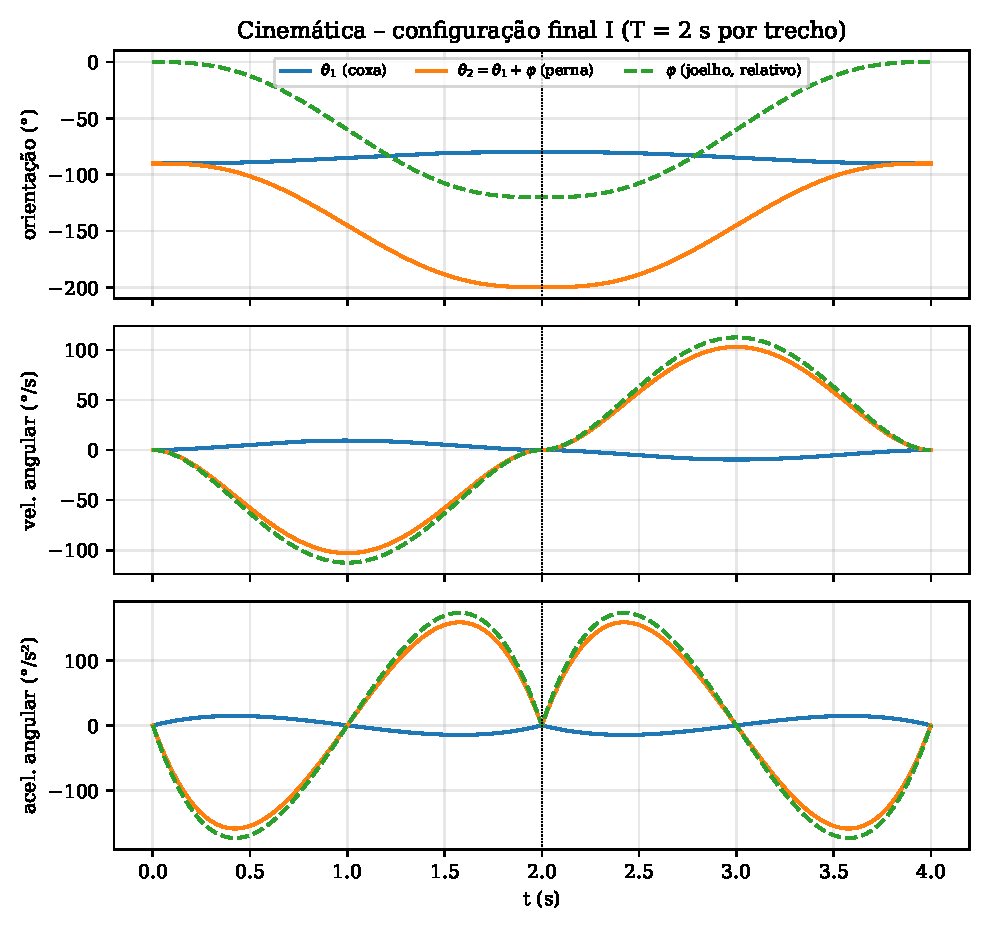
\includegraphics[width=0.85\textwidth]{figuras/p2_cinematica_I.pdf}
  \caption{Orientação, velocidade e aceleração angulares -- configuração final~I.}
  \label{fig:cinI}
\end{figure}

\begin{figure}[htbp]
  \centering
  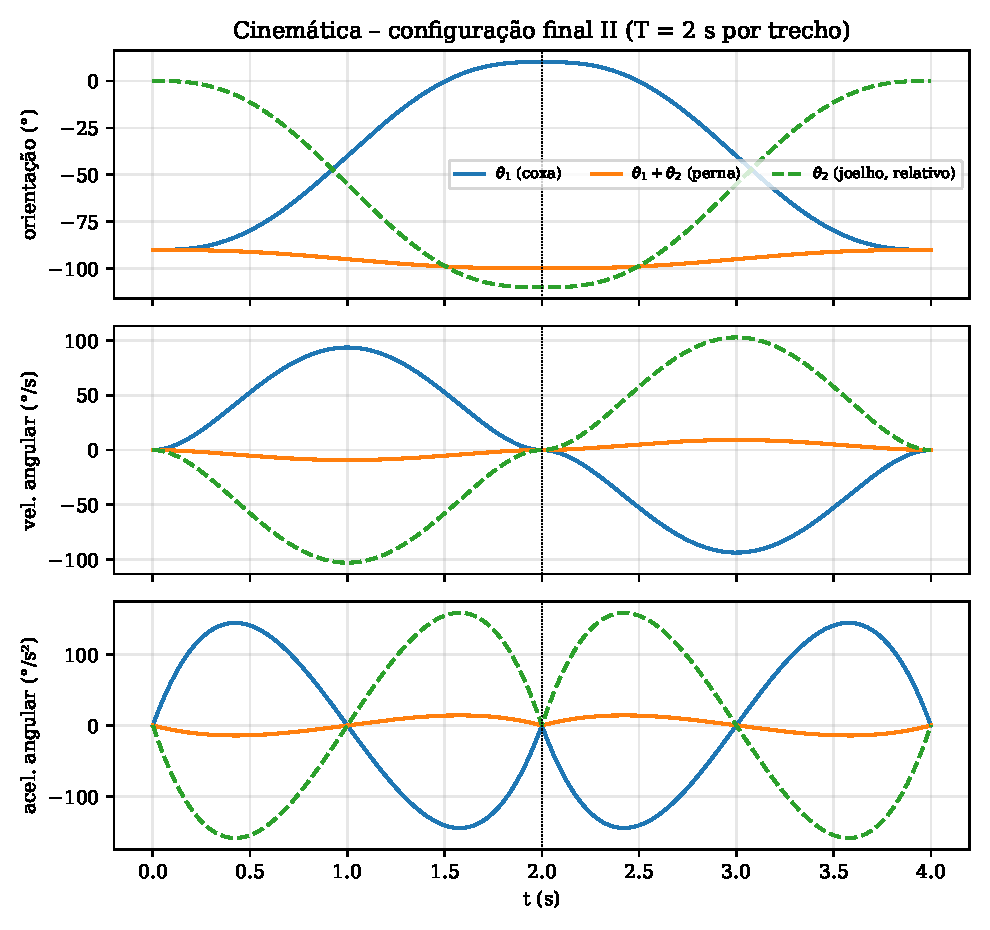
\includegraphics[width=0.85\textwidth]{figuras/p2_cinematica_II.pdf}
  \caption{Orientação, velocidade e aceleração angulares -- configuração final~II.}
  \label{fig:cinII}
\end{figure}

\begin{figure}[htbp]
  \centering
  \begin{subfigure}[b]{0.45\textwidth}
    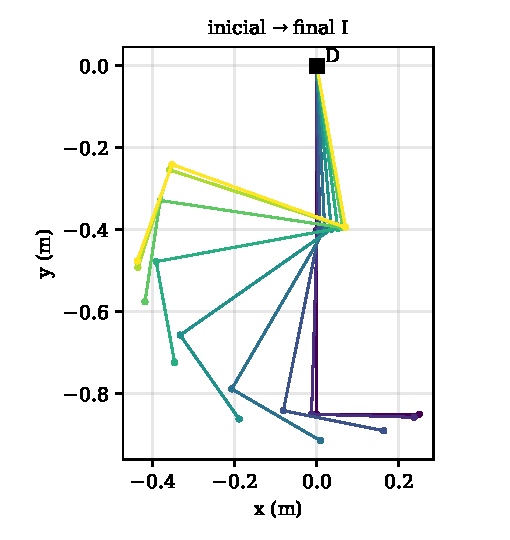
\includegraphics[width=\textwidth]{figuras/p2_estrobo_I.pdf}
  \end{subfigure}\hfill
  \begin{subfigure}[b]{0.45\textwidth}
    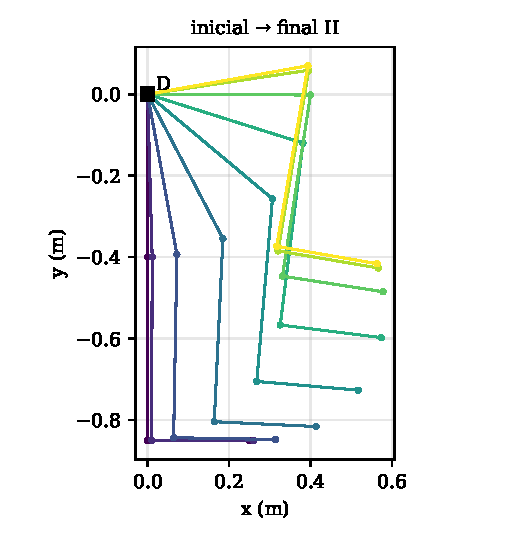
\includegraphics[width=\textwidth]{figuras/p2_estrobo_II.pdf}
  \end{subfigure}
  \caption{Instantâneos do movimento de ida (intervalos de $T/8$).}
  \label{fig:estrobo}
\end{figure}

\subsection{Torques dos atuadores}

As \cref{fig:torI,fig:torII} decompõem os torques nas parcelas gravitacional, inercial e
centrípeta/Coriolis, e a \cref{tab:torques} resume os valores máximos, os valores eficazes
(RMS, relevantes para o aquecimento dos motores) e as potências mecânicas máximas
$P = \tau\,\dot q$.

\begin{table}[htbp]
  \centering
  \caption{Torques (N\,m) e potências (W) dos atuadores, $T=\SI{2}{s}$.}
  \label{tab:torques}
  \begin{tabular}{lcrrrrrr}
    \toprule
    & & \multicolumn{3}{c}{Quadril} & \multicolumn{3}{c}{Joelho} \\
    \cmidrule(lr){3-5}\cmidrule(lr){6-8}
    Configuração & $M$ (kg) & $|\tau|_{\max}$ & $\tau_{\mathrm{RMS}}$ & $|P|_{\max}$ & $|\tau|_{\max}$ & $\tau_{\mathrm{RMS}}$ & $|P|_{\max}$ \\
    \midrule
    \tabelatorques
    \bottomrule
  \end{tabular}
\end{table}

\begin{figure}[htbp]
  \centering
  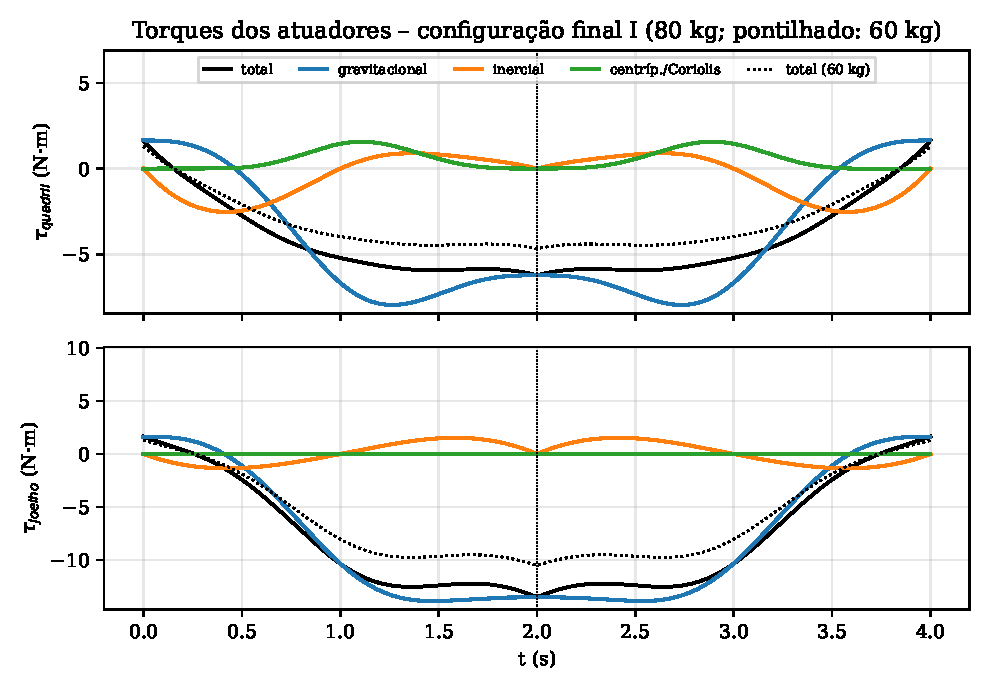
\includegraphics[width=0.9\textwidth]{figuras/p2_torques_I.pdf}
  \caption{Torques no quadril e no joelho -- configuração final~I.}
  \label{fig:torI}
\end{figure}

\begin{figure}[htbp]
  \centering
  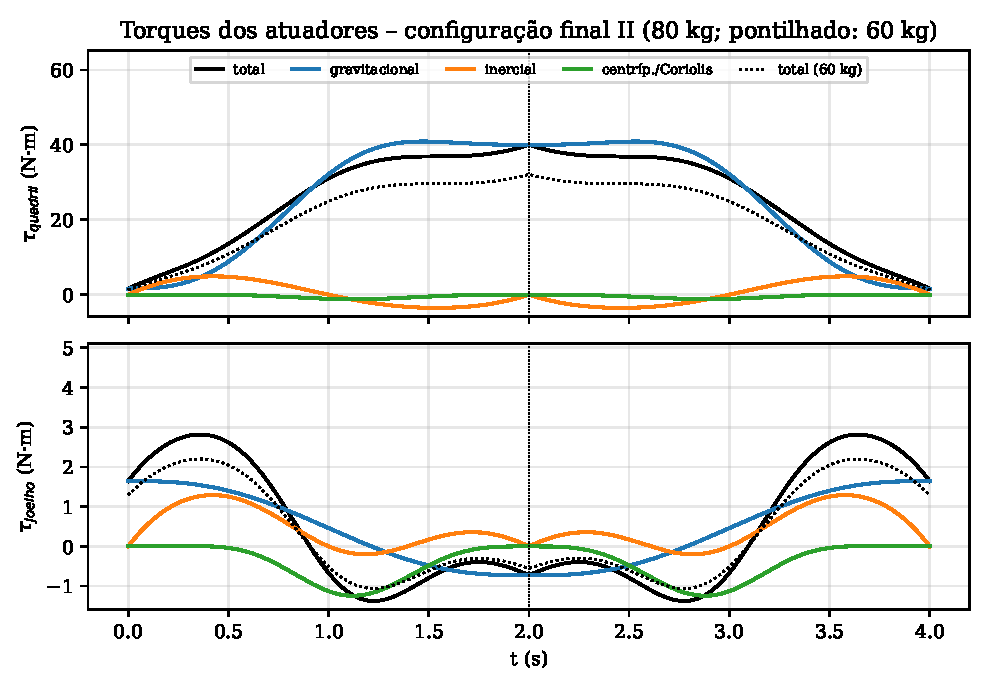
\includegraphics[width=0.9\textwidth]{figuras/p2_torques_II.pdf}
  \caption{Torques no quadril e no joelho -- configuração final~II.}
  \label{fig:torII}
\end{figure}

\paragraph{Análise.}
\begin{itemize}
  \item Na \textbf{configuração final~I}, o esforço concentra-se no joelho
  (\tjImax~N\,m): a perna e o pé, com braço de alavanca crescente à medida que a perna se
  aproxima da horizontal ($\theta_1+\theta_2 \approx \SI{-180}{\degree}$), exigem torque para vencer o
  peso. O quadril move-se apenas \SI{10}{\degree} e seu torque é pequeno.
  \item Na \textbf{configuração final~II}, o quadril é crítico (\tqIImax~N\,m), pois precisa
  sustentar a coxa na horizontal com a perna pendente: toda a massa do membro e da
  órtese tem braço de alavanca máximo. O joelho quase não trabalha, pois a perna
  permanece aproximadamente vertical ($\theta_1+\theta_2$ varia de \SI{-90}{\degree} a
  \SI{-99,8}{\degree}).
  \item Em ambos os casos a \textbf{parcela gravitacional domina}: no atuador mais
  solicitado de cada configuração (joelho em final~I, quadril em final~II), as parcelas
  inercial e de Coriolis somadas não passam de \SI{12}{\percent} do torque máximo para
  $T = \SI{2}{s}$. Nos atuadores pouco solicitados, elas representam de \SIrange{40}{50}{\percent}
  do máximo, mas não passam de \SI{2,6}{N.m} em valor absoluto.
  Isso sugere o uso de molas de compensação gravitacional ou de redutores
  irreversíveis/freios para manter posturas estáticas sem consumo de energia.
  \item A passagem de \SI{80}{kg} para \SI{60}{kg} reduz os torques em cerca de
  \SIrange{20}{25}{\percent}, um pouco menos que a redução de \SI{25}{\percent} da massa
  corporal, pois a massa da órtese não varia com o indivíduo.
\end{itemize}

\subsection{Sensibilidade ao tempo de movimento}

A \cref{tab:sens} mostra que os torques dos atuadores críticos (joelho em final~I e
quadril em final~II) independem de $T$: o máximo ocorre na configuração final, em
repouso, e é puramente gravitacional. Nos demais, as acelerações (proporcionais a
$1/T^2$) passam a contribuir significativamente para $T = \SI{1}{s}$. No quadril em
final~I, $|\tau|_{\max}$ volta a crescer para $T$ longo: o máximo ocorre no meio do
trajeto, onde a parcela inercial se opõe à gravitacional; com $T$ grande, a parcela
inercial desaparece, e o torque tende ao máximo gravitacional ao longo do caminho
(cerca de \SI{8}{N.m}).

\begin{table}[htbp]
  \centering
  \caption{Torques máximos (N\,m) em função do tempo $T$ de cada trecho ($M=\SI{80}{kg}$).}
  \label{tab:sens}
  \begin{tabular}{crrrr}
    \toprule
    & \multicolumn{2}{c}{Final I} & \multicolumn{2}{c}{Final II} \\
    \cmidrule(lr){2-3}\cmidrule(lr){4-5}
    $T$ (s) & quadril & joelho & quadril & joelho \\
    \midrule
    \tabelasens
    \bottomrule
  \end{tabular}
\end{table}

\section{Parte II -- Dimensionamento dos atuadores e verificação estrutural}\label{cap:dimensionamento}

\subsection{Especificação dos atuadores}

Com o pior caso (\SI{80}{kg}) e um fator de serviço de 1,5, as especificações de saída são:
joelho com \SI{20}{N.m} e \SI{2,0}{rad/s} (\SI{112,5}{\degree\per\s}), e quadril com
\SI{60}{N.m} e \SI{1,6}{rad/s}. Com um redutor harmônico de razão $N=100$ e rendimento
$\eta = 0{,}70$, o motor deve fornecer
\begin{equation}
  \tau_m = \frac{\tau_{\mathrm{saída}}}{N\eta},\qquad \omega_m = N\,\omega_{\mathrm{saída}},
\end{equation}
ou seja:
\begin{align*}
  \text{joelho:}\quad & \tau_m = \frac{20}{100\cdot 0{,}70} = \SI{0,29}{N.m},\qquad
     \omega_m = 100\cdot 2{,}0 = \SI{200}{rad/s} \approx \SI{1900}{rpm};\\
  \text{quadril:}\quad & \tau_m = \frac{60}{100\cdot 0{,}70} = \SI{0,86}{N.m},\qquad
     \omega_m = 100\cdot 1{,}6 = \SI{160}{rad/s} \approx \SI{1530}{rpm}.
\end{align*} Essa faixa é atendida por motores CC sem escovas de 70 a
\SI{150}{W}, compatíveis com a massa de \SI{1,2}{kg} adotada para o atuador do joelho. O
torque RMS, bem menor que o de pico, deve ser comparado ao torque contínuo do motor.

\subsection{Verificação das hastes de alumínio}

As hastes medial e lateral dividem igualmente o momento fletor transmitido pelos
atuadores. Para a seção retangular $b\times h = \qtyproduct{20 x 5}{mm}$, com flexão no plano sagital,
\begin{equation}
  W = \frac{h\,b^2}{6} = \SI{\Wmod}{mm^3},\qquad \sigma = \frac{M_f}{2W}.
\end{equation}
O carregamento é repetido, de zero a máximo, a cada ciclo; assim,
$\sigma_a = \sigma_m = \sigma/2$, e o coeficiente de segurança à fadiga é obtido pelo
critério de Goodman modificado \cite{shigley2015}:
\begin{equation}
  \frac{\sigma_a}{S_e} + \frac{\sigma_m}{S_u} = \frac{1}{n_f}.
\end{equation}
Com $W = 5\cdot 20^2/6 = \SI{333}{mm^3}$, para a haste da perna,
$\sigma = 13{,}5/(2\cdot 333\times10^{-9}) = \SI{20,3}{MPa}$, $n_y = 276/20{,}3 = 13{,}6$ e
$1/n_f = 10{,}1/96{,}5 + 10{,}1/310 = 0{,}137$, isto é, $n_f = 7{,}3$. O mesmo cálculo para a
haste da coxa ($M_f = \SI{40,0}{N.m}$) está na \cref{tab:estrutural}.

\begin{table}[htbp]
  \centering
  \caption{Verificação estrutural das hastes em Al 6061-T6.}
  \label{tab:estrutural}
  \begin{tabular}{lrrr}
    \toprule
    Haste & $\sigma_{\max}$ (MPa) & $n_y = S_y/\sigma$ & $n_f$ (Goodman) \\
    \midrule
    Perna (torque do joelho) & \sigPerna & \nyPerna & \ngPerna \\
    Coxa (torque do quadril) & \sigCoxa & \nyCoxa & \ngCoxa \\
    \bottomrule
  \end{tabular}
\end{table}

Todos os coeficientes são superiores a 2. Deve-se, contudo, verificar os furos das
articulações (concentração de tensão, $K_t\approx 2{,}5$) e considerar a carga de apoio
durante a marcha, não incluída no ciclo analisado, que pode exigir espessuras maiores
ou a substituição pelo compósito de carbono da \cref{tab:materiais}.

\section{Conclusões}

\begin{itemize}
  \item \textbf{Parte I}: as medições feitas com o \emph{Tracker} foram convertidas para a
  base da coxa e ajustadas como movimento de corpo rígido, fornecendo quatro poses da
  perna entre \SI{0}{\degree} e \phiD\si{\degree} de flexão. A síntese por três posições
  de precisão, formulada como cálculo de circuncentros dos pontos homólogos e com a
  escolha dos pivôs móveis por otimização, produziu um quadrilátero (elos de \rCL{} a
  \rQN~mm) que passa pelas três posições de precisão e erra a posição de verificação em
  apenas \errcheque~mm no tornozelo, menos que a incerteza das próprias medições. O
  mecanismo percorre toda a faixa medida sem pontos mortos, com $\mu \ge \mumin\si{\degree}$.
  \item \textbf{Parte II}: a interpolação quíntica fornece trajetórias suaves, com
  velocidade e aceleração nulas nos extremos. Os torques necessários (até
  \tqIImax~N\,m no quadril e \tjImax~N\,m no joelho para \SI{80}{kg}) são dominados pela
  gravidade, o que orienta o projeto para a compensação gravitacional. As hastes em
  Al 6061-T6 de \qtyproduct{20 x 5}{mm} atendem com folga ao ciclo analisado.
  \item \textbf{Próximos passos}: construir e ensaiar a maquete; refinar a síntese com mais
  quadros do vídeo (síntese por mínimos quadrados); incorporar o joelho policêntrico na
  órtese, evitando o desalinhamento entre as articulações humana e artificial; e incluir
  o contato com o solo na análise dinâmica.
\end{itemize}

\section{Materiais e anexos}\label{sec:anexos}

Os arquivos utilizados na aquisição e no tratamento dos dados experimentais são
disponibilizados juntamente com o relatório, incluindo o arquivo do projeto utilizado
no software \emph{Tracker}, a planilha com as coordenadas obtidas durante o rastreamento
e os programas em Python usados nas análises.

\subsection{Dados experimentais obtidos pelo \emph{Tracker}}

A tabela a seguir apresenta as coordenadas cartesianas dos onze pontos rastreados para os
\emph{frames} registrados durante o experimento. Os valores correspondem diretamente aos
dados obtidos no arquivo de saída utilizado para a organização dos resultados
experimentais.

{\small
\begin{longtable}{cc rr}
  \caption{Coordenadas dos pontos obtidas pelo \emph{Tracker}.}\label{tab:tracker}\\
  \toprule
  Frame & Ponto & $x$ (m) & $y$ (m) \\
  \midrule
  \endfirsthead
  \toprule
  Frame & Ponto & $x$ (m) & $y$ (m) \\
  \midrule
  \endhead
  \midrule
  \multicolumn{4}{r}{Continua na próxima página}\\
  \endfoot
  \bottomrule
  \endlastfoot
    234 & 1 & \ensuremath{-}0.078146 & 0.386447 \\
    234 & 2 & 0.069715 & 0.381067 \\
    234 & 3 & 0.000380 & 0.000035 \\
    234 & 4 & 0.084056 & 0.004970 \\
    234 & 5 & \ensuremath{-}0.003477 & \ensuremath{-}0.046264 \\
    234 & 6 & 0.064449 & \ensuremath{-}0.067460 \\
    234 & 7 & \ensuremath{-}0.067107 & \ensuremath{-}0.412356 \\
    234 & 8 & \ensuremath{-}0.028615 & \ensuremath{-}0.411334 \\
    234 & 9 & 0.010899 & \ensuremath{-}0.415762 \\
    234 & 10 & \ensuremath{-}0.081579 & \ensuremath{-}0.508887 \\
    234 & 11 & 0.128059 & \ensuremath{-}0.512169 \\
    307 & 1 & \ensuremath{-}0.096598 & 0.361130 \\
    307 & 2 & 0.045186 & 0.368099 \\
    307 & 3 & 0.025422 & \ensuremath{-}0.010538 \\
    307 & 4 & 0.100385 & 0.010706 \\
    307 & 5 & 0.030582 & \ensuremath{-}0.060615 \\
    307 & 6 & 0.100689 & \ensuremath{-}0.063650 \\
    307 & 7 & 0.064449 & \ensuremath{-}0.431417 \\
    307 & 8 & 0.102506 & \ensuremath{-}0.418892 \\
    307 & 9 & 0.140082 & \ensuremath{-}0.413111 \\
    307 & 10 & 0.076024 & \ensuremath{-}0.527587 \\
    307 & 11 & 0.276455 & \ensuremath{-}0.470734 \\
    390 & 1 & \ensuremath{-}0.092092 & 0.369497 \\
    390 & 2 & 0.059443 & 0.364994 \\
    390 & 3 & \ensuremath{-}0.006151 & \ensuremath{-}0.003193 \\
    390 & 4 & 0.087942 & \ensuremath{-}0.021160 \\
    390 & 5 & \ensuremath{-}0.017371 & \ensuremath{-}0.039370 \\
    390 & 6 & 0.039383 & \ensuremath{-}0.092178 \\
    390 & 7 & \ensuremath{-}0.279894 & \ensuremath{-}0.307356 \\
    390 & 8 & \ensuremath{-}0.252276 & \ensuremath{-}0.321620 \\
    390 & 9 & \ensuremath{-}0.217070 & \ensuremath{-}0.348328 \\
    390 & 10 & \ensuremath{-}0.350911 & \ensuremath{-}0.384140 \\
    390 & 11 & \ensuremath{-}0.164262 & \ensuremath{-}0.499468 \\
    423 & 1 & \ensuremath{-}0.084368 & 0.364992 \\
    423 & 2 & 0.064305 & 0.358922 \\
    423 & 3 & 0.005695 & 0.010403 \\
    423 & 4 & 0.101903 & \ensuremath{-}0.032390 \\
    423 & 5 & \ensuremath{-}0.005007 & 0.000303 \\
    423 & 6 & 0.021836 & \ensuremath{-}0.086645 \\
    423 & 7 & \ensuremath{-}0.359654 & 0.000097 \\
    423 & 8 & \ensuremath{-}0.347216 & \ensuremath{-}0.035323 \\
    423 & 9 & \ensuremath{-}0.354246 & \ensuremath{-}0.075069 \\
    423 & 10 & \ensuremath{-}0.461318 & 0.013346 \\
    423 & 11 & \ensuremath{-}0.481342 & \ensuremath{-}0.202402 \\
    456 & 1 & \ensuremath{-}0.055404 & 0.367781 \\
    456 & 2 & 0.090948 & 0.353055 \\
    456 & 3 & 0.026919 & 0.021650 \\
    456 & 4 & 0.113090 & \ensuremath{-}0.042424 \\
    456 & 5 & 0.029978 & 0.010953 \\
    456 & 6 & 0.017711 & \ensuremath{-}0.072400 \\
    456 & 7 & \ensuremath{-}0.251153 & 0.209797 \\
    456 & 8 & \ensuremath{-}0.267954 & 0.181360 \\
    456 & 9 & \ensuremath{-}0.293245 & 0.148842 \\
    456 & 10 & \ensuremath{-}0.321909 & 0.280117 \\
    456 & 11 & \ensuremath{-}0.480643 & 0.126200 \\
    561 & 1 & \ensuremath{-}0.047680 & 0.402324 \\
    561 & 2 & 0.081961 & 0.370923 \\
    561 & 3 & 0.061252 & 0.027057 \\
    561 & 4 & 0.131913 & \ensuremath{-}0.038073 \\
    561 & 5 & 0.061220 & 0.026248 \\
    561 & 6 & 0.013809 & \ensuremath{-}0.047533 \\
    561 & 7 & \ensuremath{-}0.122496 & 0.315720 \\
    561 & 8 & \ensuremath{-}0.138852 & 0.285733 \\
    561 & 9 & \ensuremath{-}0.185196 & 0.271421 \\
    561 & 10 & \ensuremath{-}0.149757 & 0.399547 \\
    561 & 11 & \ensuremath{-}0.363074 & 0.346388 \\
\end{longtable}
}

\subsection{Programas}\label{ap:codigo}



Os programas estão na pasta \texttt{scripts/} e são executados pelo \texttt{Makefile}
(\texttt{make}), que regenera figuras, tabelas e o PDF.

\begin{description}
  \item[\texttt{parte1\_sintese.py}] leitura dos dados do \emph{Tracker}; base da coxa e poses
  da perna (Procrustes); síntese por circuncentros; simulação de montagem; otimização
  dos pivôs móveis; erro na verificação, ângulo de transmissão e centroide; gabarito da
  maquete.
  \item[\texttt{parte2\_ortese.py}] parâmetros antropométricos e da órtese; trajetórias
  quínticas; dedução simbólica (SymPy) e forma fechada da dinâmica; verificação por
  Newton--Euler; análise de sensibilidade; verificação estrutural.
  \item[\texttt{gera\_valores\_tex.py}] exporta os resultados para \texttt{dados/valores.tex}.
\end{description}

Trecho central da Parte II -- cinemática pelo método matricial e dinâmica inversa:
\begin{lstlisting}[language=Python]
T01 = T_hom(th1, 0, 0)            # 0T1 = [Rot(theta1, z1) | 0]
T12 = T_hom(th2, l1, 0)           # 1T2 = [Rot(theta2, z2) | (l1, 0)]
rG2 = T01 @ T12 @ [bx, by, 1]     # [0rG2; 1] = 0T1 1T2 [2rG2; 1]

k   = bx*c2 - by*s2
M11 = I1 + m1*a1**2 + I2 + m2*(l1**2 + bx**2 + by**2 + 2*l1*k)
M12 = I2 + m2*(bx**2 + by**2 + l1*k)
M22 = I2 + m2*(bx**2 + by**2)
h   = m2*l1*(bx*s2 + by*c2)
g2  = m2*G*(bx*c12 - by*s12)
g1  = (m1*a1 + m2*l1)*G*c1 + g2
tau_quadril = M11*dd_th1 + M12*dd_th2 - h*(2*d_th1*d_th2 + d_th2**2) + g1
tau_joelho  = M12*dd_th1 + M22*dd_th2 + h*d_th1**2 + g2
\end{lstlisting}


\clearpage
\printbibliography[heading=bibintoc,title={Referências}]

\end{document}
